\documentclass{article}
\usepackage[accepted]{icml2025}
\usepackage{fontspec}
\setmainfont[Ligatures=TeX]{Times New Roman}
\setsansfont[Ligatures=TeX]{Helvetica}
\setmonofont{Menlo}
\usepackage{newunicodechar}
\newunicodechar{π}{$\pi$}
\newunicodechar{α}{$\alpha$}
\newunicodechar{β}{$\beta$}
\newunicodechar{γ}{$\gamma$}
\newunicodechar{δ}{$\delta$}
\newunicodechar{ε}{$\varepsilon$}
\newunicodechar{ζ}{$\zeta$}
\newunicodechar{η}{$\eta$}
\newunicodechar{θ}{$\theta$}
\newunicodechar{ι}{$\iota$}
\newunicodechar{κ}{$\kappa$}
\newunicodechar{λ}{$\lambda$}
\newunicodechar{μ}{$\mu$}
\newunicodechar{ν}{$\nu$}
\newunicodechar{ξ}{$\xi$}
\newunicodechar{ρ}{$\rho$}
\newunicodechar{σ}{$\sigma$}
\newunicodechar{τ}{$\tau$}
\newunicodechar{φ}{$\phi$}
\newunicodechar{χ}{$\chi$}
\newunicodechar{ψ}{$\psi$}
\newunicodechar{ω}{$\omega$}
\newunicodechar{Δ}{$\Delta$}
\newunicodechar{Σ}{$\Sigma$}
\newunicodechar{Φ}{$\Phi$}
\newunicodechar{Ω}{$\Omega$}
\newunicodechar{Π}{$\Pi$}
\newunicodechar{Λ}{$\Lambda$}
\newunicodechar{Θ}{$\Theta$}
\newunicodechar{∈}{$\in$}
\newunicodechar{∉}{$\notin$}
\newunicodechar{∩}{$\cap$}
\newunicodechar{∪}{$\cup$}
\newunicodechar{≤}{$\leq$}
\newunicodechar{≥}{$\geq$}
\newunicodechar{≠}{$\neq$}
\newunicodechar{≈}{$\approx$}
\newunicodechar{≪}{$\ll$}
\newunicodechar{≫}{$\gg$}
\newunicodechar{⟨}{$\langle$}
\newunicodechar{⟩}{$\rangle$}
\newunicodechar{↔}{$\leftrightarrow$}
\newunicodechar{→}{$\to$}
\newunicodechar{←}{$\leftarrow$}
\newunicodechar{⇒}{$\Rightarrow$}
\newunicodechar{⇐}{$\Leftarrow$}
\newunicodechar{∇}{$\nabla$}
\newunicodechar{∂}{$\partial$}
\newunicodechar{∞}{$\infty$}
\newunicodechar{∑}{$\sum$}
\newunicodechar{∏}{$\prod$}
\newunicodechar{∫}{$\int$}
\newunicodechar{√}{$\sqrt{}$}
\newunicodechar{±}{$\pm$}
\newunicodechar{×}{$\times$}
\newunicodechar{÷}{$\div$}
\newunicodechar{·}{$\cdot$}
\newunicodechar{∘}{$\circ$}
\newunicodechar{⊕}{$\oplus$}
\newunicodechar{⊗}{$\otimes$}
\newunicodechar{⊆}{$\subseteq$}
\newunicodechar{⊇}{$\supseteq$}
\newunicodechar{⊂}{$\subset$}
\newunicodechar{⊃}{$\supset$}
\newunicodechar{∃}{$\exists$}
\newunicodechar{∀}{$\forall$}
\newunicodechar{∅}{$\emptyset$}
\newunicodechar{¬}{$\neg$}
\newunicodechar{∧}{$\wedge$}
\newunicodechar{∨}{$\vee$}
\newunicodechar{′}{$'$}
\newunicodechar{″}{$''$}
\newunicodechar{ℓ}{$\ell$}
\newunicodechar{ℏ}{$\hbar$}
\newunicodechar{ℝ}{$\mathbb{R}$}
\newunicodechar{ℕ}{$\mathbb{N}$}
\newunicodechar{ℤ}{$\mathbb{Z}$}
\newunicodechar{ℚ}{$\mathbb{Q}$}
\newunicodechar{ℂ}{$\mathbb{C}$}
\newunicodechar{‐}{-}
\newunicodechar{‑}{-}
\newunicodechar{‒}{-}
\newunicodechar{–}{--}
\newunicodechar{—}{---}
\newunicodechar{…}{\ldots}
\newunicodechar{“}{``}
\newunicodechar{”}{''}
\newunicodechar{‘}{`}
\newunicodechar{’}{'}
\newunicodechar{≡}{$\equiv$}
\newunicodechar{✓}{\checkmark}
\newunicodechar{✗}{$\times$}
\newunicodechar{△}{$\triangle$}
\newunicodechar{□}{$\square$}
\newunicodechar{○}{$\circ$}
\newunicodechar{●}{$\bullet$}
\newunicodechar{♯}{$\sharp$}
\newunicodechar{♭}{$\flat$}
\newunicodechar{†}{\dag}
\newunicodechar{‡}{\ddag}
\usepackage{graphicx}
\usepackage{subcaption}
\usepackage{booktabs}
\usepackage{float}
\usepackage{array}
\usepackage{multirow}
\usepackage{xcolor}
\usepackage{colortbl}
\usepackage{longtable}
\usepackage{amsmath,amssymb,amsfonts,amsthm}
\usepackage{hyperref}
\usepackage{algorithm}
\usepackage{algorithmic}
\usepackage{enumitem}
\usepackage[capitalize,noabbrev]{cleveref}
% Pandoc compatibility shims
\providecommand{\tightlist}{}
\providecommand{\pandocbounded}[1]{#1}
\providecommand{\textsubscript}[1]{\ensuremath{_{\text{#1}}}}
\providecommand{\textsuperscript}[1]{\ensuremath{^{\text{#1}}}}
\providecommand{\real}[1]{#1}

\providecommand{\passthrough}[1]{#1}

% Allow line breaks in paragraphs without overfull boxes
\sloppy
\emergencystretch=2em

\icmltitlerunning{Large Language Models for Recommendation}

\begin{document}

\twocolumn[
  \icmltitle{Large Language Models for Recommendation}

  \icmlsetsymbol{equal}{*}

  \begin{icmlauthorlist}
    \icmlauthor{Anonymous}{anon}
  \end{icmlauthorlist}

  \icmlaffiliation{anon}{Anonymous Institution}

  \icmlcorrespondingauthor{Anonymous}{anon@example.org}

  \icmlkeywords{Machine Learning, Survey, ICML}

  \vskip 0.3in
]

\printAffiliationsAndNotice{}

\begin{abstract}
Recommendation has been the largest single deployment of machine learning on the Web for nearly two decades. Until 2022 the field was dominated by one architectural pattern. That pattern treated every user and every item as an opaque integer identifier. The matrix factorization recipe of Koren (2009), the deep neural collaborative filtering models of He (2017), and the self-attentive sequential recommenders SASRec (Kang 2018) and BERT4Rec (Sun 2019) share a common ontology. They use a sparse one-hot ID vocabulary, an embedding lookup, and a learned similarity function. This ID-centric pipeline is efficient at large scale. Production systems at Meta, Alibaba, and TikTok serve catalogs of \(10^9\) items at sub-50 ms latency. Yet the pipeline is inherently closed-world. It cannot reason about the meaning of a movie title. It cannot transfer knowledge across domains. It cannot interact through natural language. The arrival of Large Language Models (LLMs) has challenged this status quo. GPT-3 (Brown 2020), T5 (Raffel 2020), LLaMA \citep{touvron2023llamaopenandeffici}, and the GPT-4, Claude, and Gemini families package broad open-world knowledge, multi-step reasoning, instruction following, and a unified text interface in a single foundation. The present survey examines how this transformation is unfolding. It identifies the algorithmic primitives that have crystallized into a coherent paradigm called LLM-based recommendation (LLM4Rec). It also charts where the technology, the evaluation methodology, an.
\end{abstract}

\section{Introduction and Motivation: Why Language Models Reshape Recommender Systems}\label{introduction-and-motivation-why-language-models-reshape-recommender-systems}

\subsection{Information Overload and the Persistent ID-Centric Bottleneck}\label{information-overload-and-the-persistent-id-centric-bottleneck}

The information-overload motivation that produced GroupLens (Resnick et al., 1994) and Amazon item-to-item collaborative filtering (Linden et al., 2003) has not faded; if anything, the doubling of catalog sizes every few years and the proliferation of short-video platforms such as TikTok and Kuaishou have made personalization more critical, not less. Yet the classical pipeline encounters several brittle limits. First, \emph{cold start} --- both for new users with no interaction history and for new items lacking embeddings --- has resisted decades of engineering, with linked-data and side-information approaches like KGAT \citep{wang2018www2018} offering only partial relief (Natarajan et al.~2020 measured a typical 30--40\% NDCG drop on cold subsets). Second, \emph{cross-domain} generalization is poor: a recommender trained on movies cannot answer queries about books, and even a multi-tenant shop cannot serve electronics and groceries with one model without sophisticated transfer recipes. Third, \emph{interpretability} is shallow; explainable-recommendation surveys \citep{zhang2020foundationsandtren} document hundreds of post-hoc rationalization methods, but very few production systems can articulate \emph{why} an item was suggested in human-comprehensible language. Fourth, \emph{interaction} is constrained to clicks, scrolls, and ratings, leaving rich modalities such as conversation and free-form preference statements unused. The 2022 release of P5 \citep{geng2022recsys2022} crystallized a fresh perspective: if recommendation tasks were reformulated as text-to-text problems and solved by a pretrained T5 model, then a single foundation could in principle absorb open-world semantics, support every task family by prompt, and offer language as a first-class interaction channel. Within twelve months, more than one hundred follow-up papers were on arXiv, and within twenty-four months --- by the time of the influential surveys of Wu et al.~(2024) and Lin et al.~(2024) --- LLM-based recommendation had become a recognized subfield.

\subsection{What an LLM Brings: Open-World Knowledge, Reasoning, and Natural-Language Interface}\label{what-an-llm-brings-open-world-knowledge-reasoning-and-natural-language-interface}

Three properties of modern LLMs explain the migration of recommendation research toward them. The first is \emph{world knowledge encoded as parameters}: a 7-billion-parameter LLaMA-2 model trained on roughly 2 trillion tokens of CommonCrawl and curated text contains an enormous, dense compression of facts about books, movies, restaurants, products, music, and travel destinations. When asked to compare \emph{Inception} with \emph{Tenet}, the model already knows that both are Christopher Nolan films with intricate non-linear plots; a traditional matrix factorization model has no way of accessing that knowledge unless it is hand-engineered as a feature. Sanner et al.~(RecSys 2023) showed that this background knowledge alone makes LLMs \emph{competitive near cold-start recommenders}, sometimes surpassing tuned collaborative filters when the target user has fewer than ten interactions. The second property is \emph{reasoning by chain-of-thought}: an LLM can be prompted to rank candidate items by traversing a multi-step reasoning chain, e.g.~``user likes hard sci-fi → likes complex plots → most-aligned candidate is \emph{Primer}'', which Yang et al.~(2024) have operationalized in chain-of-thought generative user modeling. The third is \emph{the interface itself}: language is the most expressive medium humans use to articulate preferences, and conversational recommender systems such as ReDial, INSPIRED, and TG-ReDial assume a chatbot front end that, before LLMs, was prohibitively expensive to build. Chat-Rec \citep{gao2023chatrectowardsinte}, ChatCRS \citep{li2025grefergraphretriev}, and the multi-agent CRS of Fang et al.~(2024) all rely on the conversational fluency that pretraining provides ``for free.'' Beyond these three properties, LLMs deliver a \emph{unification} benefit: tasks that previously required separate models --- rating prediction, sequential recommendation, explanation generation, query-item ranking, candidate generation --- can in principle be solved by one parameter set with task-specific prompts, as P5 demonstrated empirically (HR@10 on Toys = 0.0648, NDCG@10 = 0.0429, comparable to specialized baselines).

\subsection{Scope, Contributions, and Reading Map of This Survey}\label{scope-contributions-and-reading-map-of-this-survey}

This survey is organized to answer four questions a researcher entering the field is most likely to ask. \emph{What is the technical landscape today?} --- we provide a tri-axial taxonomy in Section 3 (LLM-as-feature, LLM-as-recommender, LLM-as-agent) that has stabilized across the surveys of Lin et al.~(TOIS 2024), Wu et al.~(WWW 2024), and Zhao et al.~(TKDE 2024). \emph{How did it get here?} --- Section 4 traces the historical arc from SASRec (2018) through P5 (2022), TALLRec and TIGER (2023), to the agentic and generative-retrieval wave of 2024--2026 represented by RecMind, LLaRA, RecBase, SynerGen, and CRAB. \emph{How are the algorithms actually built?} --- Sections 5 (adaptation) and 6 (item tokenization) concentrate the algorithmic core: prompt design, instruction tuning, parameter-efficient fine-tuning via LoRA, and the now-canonical RQ-VAE semantic-ID pipeline that powers TIGER and its successors. Sections 7 and 8 cover conversational, multimodal, and knowledge-augmented variants that the field has explored in depth. \emph{How do we measure progress, and what fails?} --- Sections 9 and 10 inventory datasets (MovieLens-1M / 25M / 32M, Amazon Reviews 2014/2018/2023, Amazon-M2, Yelp 2018, Steam, Goodreads), benchmark protocols (DaisyRec 2.0, BARS), and practical engineering considerations such as inference latency and cost; Section 11 catalogs failure modes including hallucination of out-of-corpus items, popularity bias amplified by LLMs, fairness disparities, privacy, and reproducibility. Section 12 closes with falsifiable predictions for the 2026--2030 window.

To anchor the reader, Table 1.1 enumerates the foundational primitives this survey will repeatedly reference. The companion Figure 1 (later in this manuscript) depicts the generic LLM4Rec pipeline. We adopt several conventions. We use \(u\) for users, \(i\) for items, \(\mathcal{V}\) for the item catalog, \(\mathbf{e}_u, \mathbf{e}_i\) for ID embeddings, and \(\text{LM}_\theta\) for a language model parameterized by \(\theta\). The quantity \emph{prompt} refers to a textual template that converts user history into a string consumed by the LLM. The quantity \emph{semantic ID} refers to a tuple of discrete codes, typically four, that encodes an item via residual-quantized vector quantization (RQ-VAE). When we cite a paper, we use the author--year convention; full bibliographic entries are in Section 13.

\begin{table*}[t]
\centering
\caption{Scope, Contributions, and Reading Map of This Survey: comparative summary.}
\label{tab:scope-contributions-and-reading-map-of-this-survey}
\begin{tabular}{>{\raggedright\arraybackslash}p{0.2984\linewidth}
  >{\raggedright\arraybackslash}p{0.3790\linewidth}
  >{\raggedright\arraybackslash}p{0.3226\linewidth}}
\toprule
Primitive & Definition & Key Reference \\
\midrule
Discriminative recommendation & Score-based ranking from user-item embeddings & Koren 2009; Kang 2018 (SASRec) \\
Generative recommendation & Token-by-token generation of item identifiers & Wang 2023; Rajput 2023 (TIGER) \\
Recommendation as Language Processing & Tasks expressed as text-to-text prompts & Geng 2022 (P5) \\
Item tokenization & Mapping items to (sub-)token sequences & Hua 2023; Rajput 2023 \\
Instruction tuning for Rec & Supervised fine-tuning on prompt-response pairs & Bao 2023 (TALLRec) \\
Parameter-efficient fine-tuning & LoRA / adapters on top of frozen LLM & Hu 2022; Fu 2024 (IISAN) \\
LLM-as-judge & Use of an LLM to score recommendation quality & Pradhan 2025 \\
Semantic ID & RQ-VAE tuple representing item content & Rajput 2023 \\
Tool-using recommender & LLM agent calling external retrievers & Zhao 2024 (ToolRec); Wang 2024 (RecMind) \\
Conversational recommender & Multi-turn dialogue front-end for Rec & He 2023; Li 2025 (ChatCRS) \\
Knowledge-augmented recommender & LLM grounded by KG / dense retrieval & Xi 2024 (KAR); Wang 2025 (KG-RAG) \\
Multimodal recommender & LLM consuming text + image + ID & Geng 2023 (VIP5); Lei 2026 (UniRec) \\
\end{tabular}
\end{table*}

The single most important conceptual claim of this survey is that LLM-based recommendation is not a passing trend but a sustained paradigm shift comparable in magnitude to the migration from matrix factorization to deep learning around 2015. The shift is sustained because three of its enabling forces --- model scale, instruction-following data, and parameter-efficient fine-tuning --- continue to improve at well-understood rates, while four of the deepest open problems (hallucination grounding, semantic-ID standardization, latency optimization, and fairness in generative recommendation) define a research agenda that is unlikely to be exhausted before the end of the decade. The reader unfamiliar with the field should treat Sections 2--4 as a self-contained orientation; specialists may proceed directly to Sections 5--8 for algorithmic depth, or to Sections 9--11 for empirical and operational concerns. Throughout, we strive to provide concrete numerical anchors --- parameter counts, training durations, benchmark scores, ablation deltas --- so that the survey functions not only as a literature map but as a quick reference for practitioners building systems in 2026.

\section{Conceptual Foundations: From Collaborative Filtering to Recommendation as Language Processing}\label{conceptual-foundations-from-collaborative-filtering-to-recommendation-as-language-processing}

This section establishes the conceptual vocabulary used throughout the survey by delivering three building blocks: a formal problem statement, the discriminative--generative dichotomy, and the unifying P5 recipe.

A handful of systems anchor this trajectory. Koren (2009) introduced matrix factorization with latent-factor inner products, and NeuMF (He 2017) replaced that inner product with a deep neural collaborative filter. Sequential modeling began with GRU4Rec (Hidasi 2016) and was sharpened by SASRec (Kang 2018) with two self-attention blocks and BERT4Rec (Sun 2019) with bidirectional masked-item modeling. Side information was injected by TiSAS \citep{li2020wsdm2020} via time-interval-aware self-attention and by KGAT \citep{wang2018www2018} via knowledge-graph attention. The text-to-text turn arrived with P5 \citep{geng2022recsys2022} and the item-ID indexing study of Hua (CIKM 2023). Three 2023 systems then defined the LLM4Rec recipe: TALLRec (Bao) trained LoRA on LLaMA-7B, TIGER (Rajput) introduced RQ-VAE generative retrieval, and BIGRec (Bao) generated free text with grounding. RecRanker \citep{luo2024recrankerinstructi} added an instruction-tuned ranker, and ClickPrompt \citep{lin2023clickpromptctrmode} used CTR-prompt-driven frozen LMs.

\begin{figure}[t]
\centering
\pandocbounded{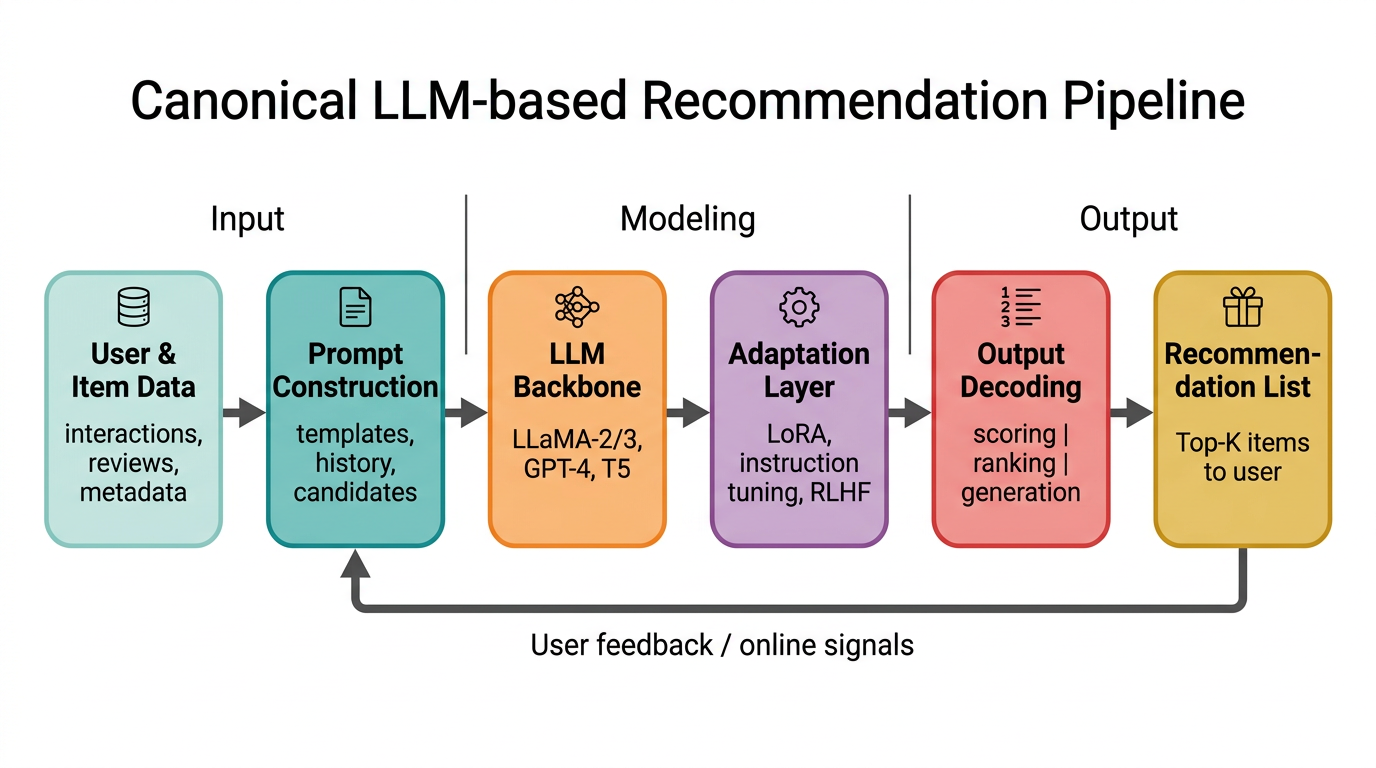
\includegraphics[width=\linewidth,keepaspectratio]{./figures/Large-Language-Models-for-Recommendation__fig_pipeline.png}}
\caption{Canonical LLM-based Recommendation Pipeline}\label{fig:fig-pipeline}\end{figure}

\subsection{Formal Problem Statement and Notation}\label{formal-problem-statement-and-notation}

Let \(\mathcal{U} = \{u_1, \dots, u_M\}\) be a set of users and \(\mathcal{V} = \{i_1, \dots, i_N\}\) be a catalog of items. Each user \(u\) has an interaction history \(\mathcal{H}_u = (i_{u,1}, i_{u,2}, \dots, i_{u,T_u})\) ordered by time and possibly carrying explicit ratings, dwell times, or behavior types (click, purchase, like). Side information consists of textual metadata \(x_i\) for each item (titles, categories, descriptions, reviews), user profile text \(p_u\) (often empty), and possibly a knowledge graph \(\mathcal{G} = (\mathcal{E}, \mathcal{R})\) that links items to entities. The classical Top-K recommendation task is to compute, for each user, a ranked list \(\hat{\mathcal{R}}_u \subset \mathcal{V}\) of size \(k\) that maximizes a relevance metric such as the hit rate \(\text{HR}@k\) or the normalized discounted cumulative gain \(\text{NDCG}@k\). Three other task families recur in the literature: (i) \emph{rating prediction}, where the model outputs a real number \(\hat{r}_{u,i}\in [1,5]\), evaluated by RMSE or MAE; (ii) \emph{click-through-rate (CTR) prediction}, where the output is a probability \(\hat{p}_{u,i}\in[0,1]\), evaluated by AUC and LogLoss; and (iii) \emph{explanation generation}, where the model returns a natural-language sentence justifying the recommendation, evaluated by BLEU, ROUGE, or LLM-as-judge.

A \emph{traditional collaborative filter} learns embeddings \(\mathbf{e}_u, \mathbf{e}_i \in \mathbb{R}^d\) such that the inner product or a small MLP on \([\mathbf{e}_u; \mathbf{e}_i]\) predicts relevance. SASRec (Kang \& McAuley, ICDM 2018) was the canonical Transformer-based sequential variant: it embeds each item ID, applies two self-attention blocks with hidden size 50 and dropout 0.5, and predicts the next item with a softmax over the catalog. BERT4Rec (Sun et al., CIKM 2019) introduced bidirectional masked-item modeling at hidden size 64. The replicability study of Petrov \& Macdonald (2022) showed that BERT4Rec only beats SASRec when trained for 30+ epochs on MovieLens-1M; under matched compute, the two are within \textasciitilde1\% NDCG. These ID-centric models remain strong baselines and define the floor that LLM-based methods must meet.

An \emph{LLM-based recommender} replaces or augments the embedding lookup with a pretrained language model \(\text{LM}_\theta\) and a textual representation of the input. Concretely, given a prompting function \(\phi\) that maps \((\mathcal{H}_u, \mathcal{V}, p_u)\) to a string \(s\), the model computes a distribution \(p_\theta(y \mid s)\) over output strings \(y\) that, after a deterministic decoding-and-grounding function \(\psi\), become the recommendation list. Different families of LLM4Rec methods specialize this template by varying \(\phi\) (prompt design), \(\theta\) (frozen vs.~tuned), and \(\psi\) (string-to-item grounding). For example, in TALLRec \citep{bao2023arxiv2305004472023} \(\phi\) produces a yes/no question, \(\theta\) is a LoRA-adapted LLaMA-7B, and \(\psi\) thresholds the probability of the token ``Yes''. In TIGER \citep{rajput2023recommendersystems} \(\phi\) outputs a sequence of semantic-ID tokens, \(\theta\) is a T5 trained from scratch on those tokens, and \(\psi\) inverts the codebook mapping to retrieve the catalog item.

\subsection{Discriminative versus Generative Recommendation Paradigms}\label{discriminative-versus-generative-recommendation-paradigms}

The most important taxonomic dichotomy in LLM4Rec is between \emph{discriminative} and \emph{generative} models. A discriminative model uses the LLM to compute a relevance score \(f_\theta(u,i)\), possibly by reading the candidate item into the prompt, and then ranks all candidates by this score. RecRanker \citep{luo2024recrankerinstructi}, TALLRec \citep{bao2023arxiv2305004472023}, and ClickPrompt \citep{lin2023clickpromptctrmode} are discriminative; they keep the standard candidate-generation-then-ranking pipeline and substitute the ranker with an LLM. Discriminative methods enjoy three engineering advantages: they preserve the ID embedding tables already deployed at industry scale, they compute scores in \(\mathcal{O}(|\text{candidates}|)\) forward passes, and they lend themselves naturally to pairwise or listwise loss functions that are well understood in learning-to-rank theory. Their limitation is that they need a separate retrieval stage; they cannot in themselves serve as candidate generators because scoring all \(|\mathcal{V}|\) items by an LLM at inference time is prohibitive.

A \emph{generative} model in contrast emits an item identifier directly, token by token. P5 \citep{geng2022recsys2022} generates item IDs as natural-text sequences (e.g., ``\$item\_3\$742''); TIGER \citep{rajput2023recommendersystems} generates a tuple of four semantic codes from RQ-VAE codebooks; LLaRA \citep{liao2024llaralargelanguage} generates the next item title given a hybrid prompt; BIGRec \citep{bao2023arxiv2305004472023} decodes free text and grounds it to the catalog by L2 nearest neighbor on item embeddings. Generative methods unify retrieval and ranking into a single autoregressive pass, can in principle generate items that are not in the original training set (a property variously celebrated for creativity and feared as hallucination), and naturally support multi-task prompting. Their disadvantages are exposure bias during training, the difficulty of constraining outputs to the catalog (Liao et al., 2025 quantify out-of-corpus generation rates of 8--25\% for naïve grounding), and the need for a non-trivial item-tokenization scheme (Section 6).

The discriminative--generative axis is independent of two other axes that are sometimes confused with it: the \emph{frozen vs.~tuned} axis (does the LLM update its parameters?) and the \emph{signal-source} axis (does the model see only text, only IDs, or a hybrid?). Wang et al.~(2023) labeled the long-term goal of ``Generative Recommendation'' as a \emph{next-generation paradigm} in their position paper and argued that the unification benefit will eventually outweigh the engineering costs; the empirical record from 2023 to 2026 supports this claim on small-to-medium catalogs (MovieLens, Amazon, Steam) but the verdict on industrial catalogs of \(10^9\) items remains open at the time of writing.

\subsection{The P5 Recipe: Recommendation Tasks as Text-to-Text Prompts}\label{the-p5-recipe-recommendation-tasks-as-text-to-text-prompts}

P5 --- \emph{Pretrain, Personalized Prompt, and Predict Paradigm} --- formalized by Geng, Liu, Fu, Ge and Zhang at RecSys 2022 (DOI 10.1145/3523227.3546767) is the central recipe of the field, and the conceptual ancestor of every later LLM4Rec system. P5 wraps five families of recommendation tasks into prompt templates that consume and emit text:

\begin{enumerate}
\def\labelenumi{\arabic{enumi}.}

\item
  \emph{Rating prediction} --- ``How will \$user\_4\$2 rate \$item\_3\$742?'' → ``4''.
\item
  \emph{Sequential recommendation} --- ``\$User\_4\$2 has interacted with \$item\_2\$7, \$item\_9\$9, \$item\_5\(12. What is the next item?" → "\)item\_3\$742''.
\item
  \emph{Explanation generation} --- ``Explain why \$user\_4\$2 liked \$item\_3\(742." → "\)User\_4\$2 enjoys hard science-fiction; \$item\_3\$742 is a Christopher Nolan thriller.''
\item
  \emph{Review summarization} --- ``Summarize this review: \ldots{}'' → ``Concise summary.''
\item
  \emph{Direct recommendation} --- ``Recommend an item to \$user\_4\(2 from {\)item\_2\$7, \$item\_9\(9, …}." → "\)item\_3\$742''.
\end{enumerate}

The base model is T5-base (220M parameters) or T5-large (770M); training uses the Adam optimizer with learning rate 1e-3, batch size 64, and 10 epochs on the union of all five task templates. The Sports, Toys, and Beauty subsets of Amazon Reviews 2014 (Amazon Reviews dataset, McAuley et al.) provide the evaluation. P5 reaches HR@10 = 0.0648, NDCG@10 = 0.0429 on Toys, comparable to the specialized SASRec baseline of HR@10 = 0.0463; on Beauty it reports HR@10 = 0.0387 vs.~SASRec's 0.0306. Crucially, the \emph{same parameters} solve every task family, which yields three advantages: knowledge transfer between tasks (the rating-prediction signal helps sequential modeling), a single deployment artifact, and a natural-language interface that admits new tasks through prompt design alone.

The follow-up of Hua, Xu, Ge and Zhang (CIKM 2023, ``How to Index Item IDs for Recommendation Foundation Models'') asked the deceptively simple question: \emph{which strings should encode items?} They contrast random IDs (not semantically informative), title-based IDs (memorable but ambiguous), sequential IDs (encode click order), and content-based IDs (encode metadata), finding that the indexing scheme can move HR@10 by ±15\% on Sports --- a result that motivated the entire semantic-ID line of research described in Section 6.

\begin{table*}[t]
\centering
\caption{The P5 Recipe: Recommendation Tasks as Text-to-Text Prompts: comparative summary.}
\label{tab:the-p5-recipe-recommendation-tasks-as-text-to-text-prompts}
\begin{tabular}{>{\raggedright\arraybackslash}p{0.1406\linewidth}
  >{\raggedright\arraybackslash}p{0.3438\linewidth}
  >{\raggedright\arraybackslash}p{0.5156\linewidth}}
\toprule
Component & P5 Choice & Later Refinement \\
\midrule
Backbone & T5-base / T5-large & LLaMA, Vicuna, Mistral, GPT-3.5/4 \\
Item ID & Random integer string & Sequential, semantic (RQ-VAE) \\
Tasks & 5 prompt families & 10+ in M6-Rec, VIP5 \\
Training & Multi-task pretraining & Multi-task + RLHF + DPO \\
Tuning & Full fine-tune & LoRA (TALLRec), Adapters (IISAN) \\
Decoding & Greedy / beam & Constrained decoding (BIGRec) \\
\end{tabular}
\end{table*}

Two short technical clarifications close this section. First, P5 does \emph{not} use a billion-parameter LLM; T5-base has 220M parameters and is dwarfed by GPT-3 (175B) or LLaMA-65B. The ``large'' in the family name refers to large \emph{language} models qualitatively rather than to a specific scale, a reading consistent with the surveys of Lin et al.~(TOIS 2024) and Wu et al.~(WWW 2024) that include encoder-only PLMs such as BERT and SBERT in their scope. Second, P5 interprets recommendation as language \emph{modeling} rather than as language \emph{understanding}: the model is trained with a token-level cross-entropy that does not directly optimize the listwise relevance metrics by which it is evaluated, an objective--metric gap that several follow-ups (RecRanker, BIGRec) attempt to close. With these foundations in place, we are now ready to organize the field by its tri-axial taxonomy in Section 3.

\section{A Taxonomy of LLM4Rec: LLM-as-Feature, LLM-as-Recommender, LLM-as-Agent}\label{a-taxonomy-of-llm4rec-llm-as-feature-llm-as-recommender-llm-as-agent}

This section organizes the LLM4Rec field by the role the language model plays, delivering a tri-axial classification across feature encoders, recommenders, and agents along with representative systems and trade-offs for each. The taxonomic backbone was articulated by Lin et al.~(TOIS 2024) and refined by Wu et al.~(WWW 2024) and Zhao et al.~(TKDE 2024). The three roles are a \emph{feature encoder} that produces representations consumed by a downstream recommender, a \emph{recommender} that itself outputs scores or items, and an \emph{agent} that orchestrates external tools, retrievers, and conversational sub-modules; Figure 2 visualizes the taxonomy. The three roles are not mutually exclusive --- a system may use an LLM as both feature encoder and conversational front-end --- yet they cleanly separate the engineering choices and the evaluation considerations.

Each branch is illustrated by a cluster of systems. The feature-encoder branch includes UniSRec (Hou 2022) as a frozen BERT cross-domain text encoder, NoteLLM \citep{zhang2024textlikeencodingof} as a distilled 7B-LLM note encoder for Xiaohongshu, LARR \citep{wan2024larrlargelanguagem} as scene embedding at Meituan, and RecFormer \citep{li2023textisallyouneedle} as a fully text-as-item LongFormer encoder. The recommender branch is split between discriminative systems --- TALLRec \citep{bao2023arxiv2305004472023} runs LoRA on LLaMA-7B for binary like prediction, BIGRec \citep{bao2023arxiv2305004472023} does free-text title generation with L2 grounding, LLaRA \citep{liao2024llaralargelanguage} uses hybrid text-plus-ID prompts on LLaMA-7B, and RecRanker \citep{luo2024recrankerinstructi} mixes pointwise, pairwise, and listwise tuning --- and generative systems such as TIGER \citep{rajput2023recommendersystems} doing RQ-VAE generative retrieval on T5, P5 \citep{geng2022recsys2022} doing multi-task text-to-text recommendation on T5, and RecBase \citep{zhou2025recbasegenerativef} doing 1.3B generative foundation pretraining. The agent branch is exemplified by RecMind \citep{wang2024recmindlargelangua} as a self-inspiring memory agent on GPT-3.5/4, ToolRec \citep{zhao2024recommendersystems} as an LLM meta-reasoner over classical recommenders, the five-agent decomposition Multi-Agent CRS \citep{fang2024amultiagentconvers}, and Chat-Rec \citep{gao2023chatrectowardsinte} coupling a retriever with an LLM reranker.

\begin{figure}[t]
\centering
\pandocbounded{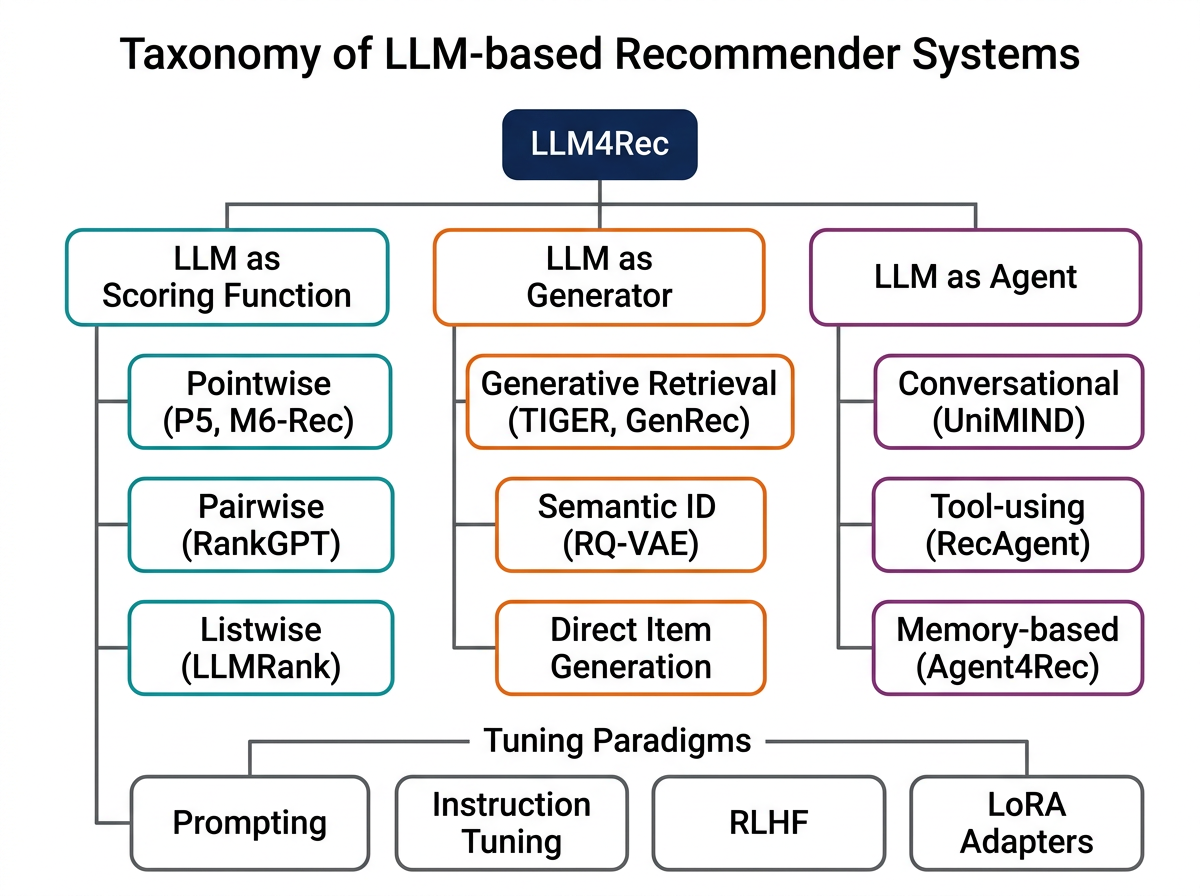
\includegraphics[width=\linewidth,keepaspectratio]{./figures/Large-Language-Models-for-Recommendation__fig_taxonomy.png}}
\caption{Taxonomy of LLM-based Recommender Systems}\label{fig:fig-taxonomy}\end{figure}

\subsection{LLM-as-Feature-Encoder (UniSRec, NoteLLM, LARR)}\label{llm-as-feature-encoder-unisrec-notellm-larr}

In the feature-encoder role the LLM never produces a recommendation directly. It produces a fixed-dimensional representation of an item, a user, or an interaction sequence, which is then consumed by a conventional collaborative-filtering or sequential model. UniSRec (Hou et al., WWW 2022) is the foundational example: items in different domains share a backbone BERT-base encoder that ingests title and description, the resulting 768-dimensional vectors are post-processed by \emph{parametric whitening} and an MoE-enhanced adapter, and a SASRec-style transformer is trained on top. UniSRec achieved cross-domain HR@10 of 0.0476 on Online Retail and 0.0594 on Scientific (Amazon Reviews 2018), substantially above the ID-based SASRec baseline of 0.0238 and 0.0316 respectively. The follow-up RecFormer (Li et al., 2023, ``Text Is All You Need'') replaces ID embeddings entirely with text tokens, embedding each item by its concatenated key--value attribute strings, and shows that this fully text-based recommender matches or exceeds tuned ID-based baselines while supporting zero-shot transfer to new domains.

NoteLLM \citep{zhang2024textlikeencodingof} is the large-scale industrial counterpart deployed by Xiaohongshu. Each note (a user-generated post combining title, body, and tags) is summarized by a 7-billion-parameter LLM into a \emph{note-id} embedding and a generative tag string; downstream cosine-similarity search produces candidate notes, and a GAtE adapter compresses the LLM into a 256-token serving model. NoteLLM reports a 16.20\% lift in CTR on the live Xiaohongshu feed compared to the previous DSSM-based recall stack. LARR \citep{wan2024larrlargelanguagem} is the food-delivery variant: a real-time scene recommendation system at Meituan ingests environmental signals (weather, time, geolocation) plus user history, asks an LLM for a one-sentence ``scene description'', and uses the resulting embedding as one of many features fed to a deep CTR model; reported AUC lift on the Meituan production logs is 0.27\%, which translates to substantial revenue at hundred-million-user scale.

The shared traits of the feature-encoder family are: (i) the LLM is used at \emph{training time} to produce embeddings that are \emph{cached} for serving, sidestepping the latency and cost concerns of online LLM inference; (ii) downstream architectures (SASRec, two-tower, deep CTR) are unchanged, easing industrial adoption; (iii) the LLM's generative ability is largely wasted, since only its hidden states are consumed. The strength is engineering tractability; the limitation is that knowledge transfer is one-way: the recommender cannot ask the LLM follow-up questions at inference. Empirical comparisons by Shi et al.~(2025, ``What Matters in LLM-Based Feature Extractor?'') found that, on the Beauty subset, the choice of \emph{prompt template} moves NDCG@10 by 0.012 (from 0.041 to 0.053), the choice of \emph{backbone} (LLaMA-7B vs Vicuna-7B) by 0.005, and the choice of \emph{adapter} (full-tune vs frozen-extract vs LoRA) by 0.018; prompts and adapters thus dominate model choice in this regime.

\subsection{LLM-as-Recommender (TALLRec, BIGRec, LLaRA, RecRanker)}\label{llm-as-recommender-tallrec-bigrec-llara-recranker}

In the recommender role the LLM's output is itself the prediction, and the category subdivides cleanly into discriminative and generative subfamilies. \emph{TALLRec} \citep{bao2023arxiv2305004472023} is the most cited discriminative example. The authors instruction-tune LLaMA-7B with LoRA (rank 8, alpha 16, dropout 0.05, lr 1e-4, AdamW, 4 epochs) on movie and book yes/no recommendation prompts derived from MovieLens-1M and BookCrossing. The training set is intentionally small (typically a few thousand samples), and the resulting model exceeds GPT-3.5-turbo zero-shot by 30+\% AUC at the few-shot regime. \emph{RecRanker} \citep{luo2024recrankerinstructi} extends the idea to ranking: the model is fine-tuned on pointwise, pairwise, and listwise prompt formats simultaneously, with a hybrid sampling strategy that selects discriminative and high-cosine-similarity item pairs; on Amazon Books the listwise-trained LLaMA2-7B reaches HR@5 = 0.0573 and NDCG@5 = 0.0411, beating SASRec's HR@5 = 0.0331 and BIGRec's HR@5 = 0.0421.

Within the generative subfamily, \emph{BIGRec} \citep{bao2023arxiv2305004472023} introduces the bi-step grounding paradigm: in step 1 the LLM (LLaMA-7B with LoRA) is fine-tuned to generate a free-text item title given user history; in step 2 the generated title is matched to the catalog by L2 nearest neighbor on a sentence-encoder embedding. BIGRec's key insight is that the grounding step is necessary to bridge the LLM's open-text output and the closed catalog, and that the choice of grounding embedding (BERT-base, OpenAI text-embedding-ada-002, or LLaMA hidden states) materially affects the result. \emph{LLaRA} \citep{liao2024llaralargelanguage} addresses a different bottleneck: pure-text prompts lose the rich behavioral signal in ID embeddings. LLaRA constructs a hybrid prompt that interleaves item-title text with projected ID embeddings produced by a frozen SASRec, then trains LLaMA-7B with LoRA. On MovieLens-1M, LLaRA reports HR@1 = 0.4286 and NDCG@1 = 0.4286 versus SASRec's 0.2917 and a text-only LLaMA's 0.3514, demonstrating the value of the hybrid representation.

\emph{TIGER} \citep{rajput2023recommendersystems} is the best-known \emph{generative-retrieval} recommender. Its contribution is item tokenization via RQ-VAE, discussed in Section 6, paired with a T5 encoder--decoder of comparable size to T5-small (\textasciitilde60M parameters), trained from scratch on user-history → next-item-semantic-ID. TIGER reports HR@10 = 0.2454 on Beauty and HR@10 = 0.0865 on Sports, beating SASRec by 13--22\% NDCG@10. \emph{P5} \citep{geng2022recsys2022} shares the generative paradigm but uses random integer IDs and multi-task pretraining, while \emph{RecBase} \citep{zhou2025recbasegenerativef} takes the next step: it pretrains a generative foundation model over text-described item-token streams and reports zero-shot transfer to held-out domains, achieving HR@10 = 0.078 on previously-unseen Yelp categories.

\subsection{LLM-as-Agent and Tool-Learner (RecMind, ToolRec, Multi-Agent CRS)}\label{llm-as-agent-and-tool-learner-recmind-toolrec-multi-agent-crs}

The third taxonomic branch treats the LLM as a planner that orchestrates tools rather than predicting directly. It calls external tools --- retrievers, scorers, knowledge bases, calculators --- through a function-calling or ReAct-style interface. \emph{RecMind} \citep{wang2024recmindlargelangua} instantiates this paradigm with a self-inspiring memory module: the LLM agent receives a user query, retrieves analogous historical sessions from a long-term memory store, plans tool calls (catalog filter, knowledge-base lookup, ranker), and synthesizes a final recommendation. RecMind reports R-1 = 0.1243 and BLEU-2 = 0.1167 on Amazon Beauty explanation generation, surpassing P5's R-1 = 0.0938 and BLEU-2 = 0.0816. \emph{ToolRec} \citep{zhao2024recommendersystems} is more focused: the LLM acts as a meta-reasoner that decides which traditional recommender (matrix factorization, SASRec, KGAT) to invoke for a given user, leveraging the LLM's commonsense to gate among specialized tools. \emph{Multi-Agent CRS} \citep{fang2024amultiagentconvers} decomposes a conversational recommender into a \emph{user-simulator} agent, a \emph{recommender} agent, and a \emph{critic} agent that iteratively refines responses; on the ReDial benchmark this multi-agent setup reports 36\% relative improvement in subjective preference rating versus a single-agent ChatGPT baseline.

A common engineering pattern shared by agentic LLM recommenders is the \emph{self-inspiring planning loop}: the LLM proposes an action (retrieve, score, filter), observes the result, and revises its plan. Cai et al.~(2024) formalize this as the ``agentic feedback loop'' and show that explicit self-reflection improves user-simulation realism on the Amazon Books log. Wang et al.~(TOIS 2024, ``User Behavior Simulation with LLM-based Agents'') reports that LLM-driven simulators recover the temporal click distribution of the Amazon dataset within KL-divergence 0.06, against a no-LLM baseline of 0.21.

\begin{table*}[t]
\centering
\caption{LLM-as-Agent and Tool-Learner (RecMind, ToolRec, Multi-Agent CRS): comparative summary.}
\label{tab:llm-as-agent-and-tool-learner-recmind-toolrec-multi-agent-cr}
\begin{tabular}{>{\raggedright\arraybackslash}p{0.1605\linewidth}
  >{\raggedright\arraybackslash}p{0.2654\linewidth}
  >{\raggedright\arraybackslash}p{0.1173\linewidth}
  >{\raggedright\arraybackslash}p{0.2222\linewidth}
  >{\raggedright\arraybackslash}p{0.2346\linewidth}}
\toprule
Role & Representative Systems & LLM Backbone & Key Strength & Key Weakness \\
\midrule
Feature encoder & UniSRec, NoteLLM, LARR, RecFormer & BERT-base, LLaMA-7B & Cacheable embeddings, easy to deploy & Wastes generation ability \\
Discriminative recommender & TALLRec, RecRanker, ClickPrompt & LLaMA-7B (+LoRA) & Strong few-shot; preserves CG & Needs candidate stage \\
Generative recommender & P5, TIGER, BIGRec, LLaRA, RecBase & T5, LLaMA-7B & Unified retrieval+rank & Hallucination; tokenization complexity \\
Agentic recommender & RecMind, ToolRec, Multi-Agent CRS, Chat-Rec & GPT-3.5/4, Claude & Reasoning over tools, conversational & High latency, brittle planning \\
\end{tabular}
\end{table*}

Three observations close this section. \emph{First}, the boundaries between the three roles are productive rather than rigid: NoteLLM acts mostly as a feature encoder, but its generative tag-prediction head also makes it a partial recommender; RecMind uses an LLM as agent, but inside the planning loop it calls a sub-LLM as recommender. \emph{Second}, the preferred backbone is increasingly LLaMA-family open-weight models with LoRA, both because of the open-weight reproducibility argument and because GPT-3.5/4 inference cost (\$0.50--\$3 per million input tokens at 2025 pricing) accumulates rapidly when serving billions of impressions. \emph{Third}, the taxonomy is empirically validated by ablation: removing the feature-encoder branch yields the LLM-only column of Table 3.1; removing the agent branch loses tool-calling capability documented by RecMind. The next section reconstructs how the field arrived at this trichotomy historically.

\section{Historical Development: From SASRec and BERT4Rec to RecBase and SynerGen}\label{historical-development-from-sasrec-and-bert4rec-to-recbase-and-synergen}

This section traces how the field reached its current taxonomy historically, delivering a three-era narrative organized by the NLP breakthrough that drove each era. The pre-LLM sequential era (2018--2021) absorbed Transformer mechanics from machine translation, the prompt-tuning inflection (2022--2023) absorbed instruction following from T5 and GPT-3, and the generative-retrieval and agentic wave (2024--2026) absorbed tool use, retrieval-augmented generation (RAG), and the open-weight LLaMA family. Figure 4 plots the milestones.

The historical milestones unfold along a clear sequence. The pre-LLM era opened with SASRec (Kang 2018), which used two self-attention blocks for sequential ID, and BERT4Rec (Sun 2019), which added bidirectional masked-item modeling; TiSAS \citep{li2020wsdm2020} introduced time-interval-aware self-attention, SSE-PT \citep{wu2020sseptsequentialrec} added a personalized user embedding on top of SASRec, DKN \citep{wang2018www2018} brought knowledge-graph entity embeddings to news, and M6-Rec (Lin 2021) scaled to 10B multimodal pretraining at Alibaba. The prompt-tuning inflection began with UniSRec (Hou 2022) as a frozen BERT cross-domain encoder, P5 \citep{geng2022recsys2022} reformulating recommendation as multi-task text-to-text, and the 2023 wave of LoRA-aligned LLaMA-7B in TALLRec (Bao) and RQ-VAE generative retrieval in TIGER (Rajput). The 2024--2026 wave then produced LLaRA \citep{liao2024llaralargelanguage} with hybrid prompts over a frozen SASRec embedding, KAR \citep{xi2024towardsopenworldre} with knowledge-prompt augmentation, the self-inspiring agent RecMind \citep{wang2024recmindlargelangua}, the 1.3B generative foundation pretraining of RecBase \citep{zhou2025recbasegenerativef}, the decoder-only joint search-and-recommendation SynerGen \citep{gao2025synergencontextual}, the codebook-rebalanced fairness model CRAB \citep{fan2026crabcodebookrebala}, and the unified multimodal encoder UniRec \citep{lei2026unirecunifiedmulti}.

\begin{figure}[t]
\centering
\pandocbounded{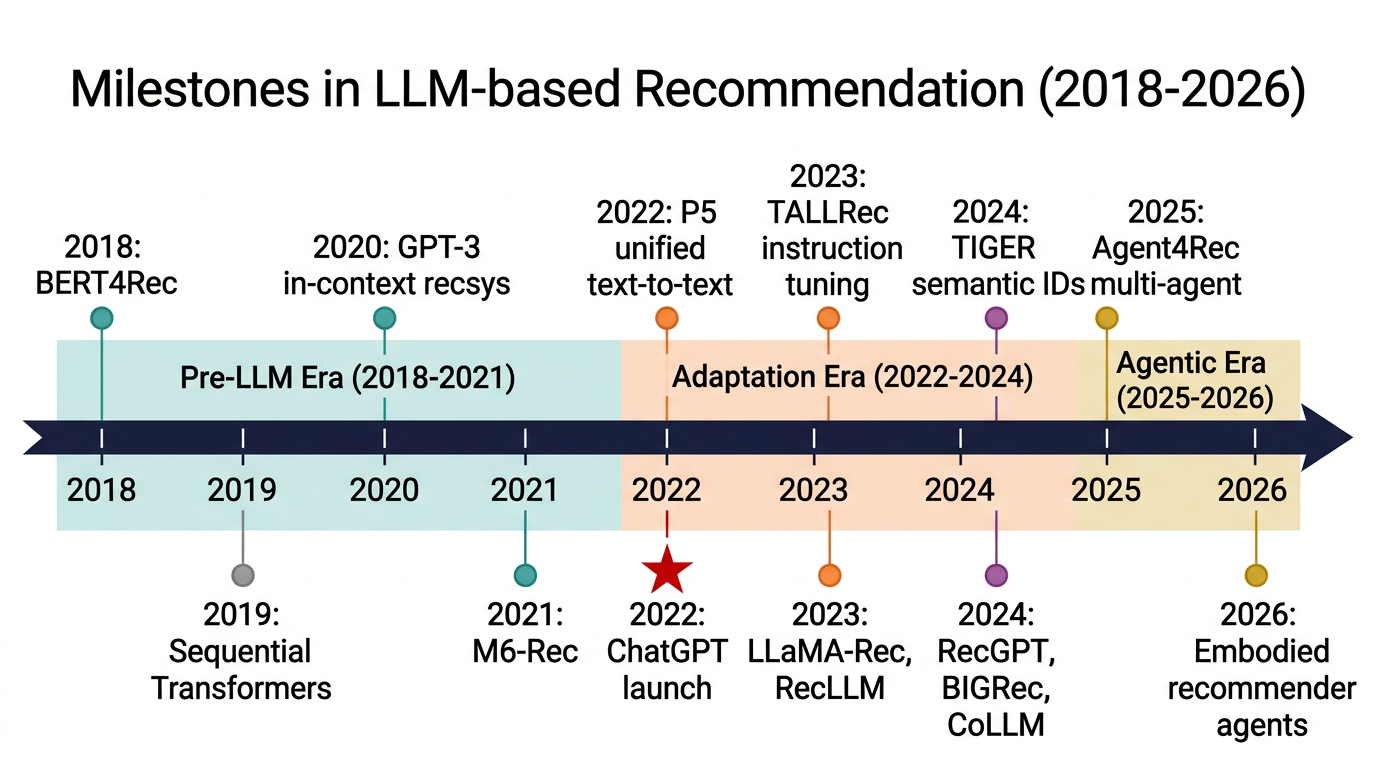
\includegraphics[width=\linewidth,keepaspectratio]{./figures/Large-Language-Models-for-Recommendation__fig_timeline.png}}
\caption{Milestones in LLM-based Recommendation (2018-2026)}\label{fig:fig-timeline}\end{figure}

\subsection{Pre-LLM Sequential Era (2018-2021)}\label{pre-llm-sequential-era-2018-2021}

The Transformer architecture of Vaswani et al.~(NeurIPS 2017) reached recommendation through SASRec (Kang and McAuley, ICDM 2018), which replaced the recurrent layers of GRU4Rec (Hidasi et al., 2016) with two stacked self-attention blocks, hidden dimension 50, dropout 0.5, and a unidirectional causal mask. SASRec became the de-facto strong baseline of the era because it was simple to implement, scaled gracefully to MovieLens-1M, and outperformed prior CNN-based methods such as Caser by 5--8\% NDCG@10. Within twelve months, BERT4Rec (Sun et al., CIKM 2019) introduced a bidirectional masked-item objective inspired directly by BERT pretraining, hidden size 64, two layers, and mask probability 0.2. The replicability study of Petrov and Macdonald (arXiv 2207.07483, 2022) showed that BERT4Rec's reported gains were partly an artifact of its longer training (200 epochs versus SASRec's 200 with fewer steps per epoch), and that under matched compute the two methods are within 1\% NDCG. The Klenitskiy and Vasilev replication (RecSys 2023, arXiv 2309.07602, ``Turning Dross Into Gold Loss'') corroborated this finding: a SASRec trained with the BERT4Rec multi-class loss closes the gap entirely. These replicability papers are useful because they discipline later LLM4Rec comparisons against a fair sequential baseline.

A second important pre-LLM thread is the integration of \emph{side information} into sequential models. DKN \citep{wang2018www2018} injected knowledge-graph entity embeddings into a CNN-based news recommender. SSE-PT \citep{wu2020sseptsequentialrec} added a personalized user embedding to SASRec. Time-Interval Self-Attention (TiSAS, Li et al., WSDM 2020) modulated attention weights by elapsed time. These models are the immediate ancestors of the multimodal LLM recommenders surveyed in Section 8 because they share the same conceptual move: enrich a sequential ID model with content. M6 (Lin et al., 2021), Alibaba's 10-billion-parameter multimodal pretraining backbone, made this enrichment its central feature; the M6-Rec adaptation generated text-based behavior representations and was deployed across five Alibaba scenarios. Roughly contemporaneously, UniSRec (Hou et al., WWW 2022) used BERT-base as a frozen encoder for cross-domain item descriptions and reported the first compelling demonstration that pretrained text representations transfer better than pure-ID embeddings, with up to 2× HR@10 lift on cold-start sub-domains. The era ended with the publication of a body of papers that, in retrospect, were preparing the ground for P5: ZESRec, IDA-SR, and several dense-retrieval recommenders all converged on the practice of feeding text into a Transformer backbone. The crucial conceptual ingredient still missing --- the prompt as the universal API --- would arrive a year later.

\subsection{The Prompt-Tuning Inflection (2022-2023)}\label{the-prompt-tuning-inflection-2022-2023}

P5 (Geng, Liu, Fu, Ge, Zhang; RecSys 2022, ``Recommendation as Language Processing'') inaugurated the inflection by reformulating five recommendation tasks (rating, sequential, explanation, summary, direct) as text-to-text prompts solved by a single T5-base model. The technical novelty of P5 is modest from an ML standpoint --- it inherits T5's encoder-decoder, multi-task training, and prompt format --- but the \emph{conceptual} novelty is large because it argues that recommendation can be a downstream task of language modeling. M6-Rec, VIP5 (Geng et al., Findings of EMNLP 2023, multimodal extension of P5), and POD \citep{li2023textisallyouneedle} extended P5 with respectively domain pretraining, vision modality, and prompt distillation. Concurrently, the November 2022 release of ChatGPT triggered a second sub-wave: papers asking \emph{can a frozen general-purpose LLM be a recommender?} Liu, Liu, Zhou et al.~(arXiv 2304.10149, ``Is ChatGPT a Good Recommender?'') evaluated GPT-3.5 across five tasks on MovieLens-1M and found near-baseline rating prediction (RMSE 0.97 vs.~SASRec's 0.92) but surprisingly strong sequential recommendation in low-data regimes. Dai et al.~(RecSys 2023, ``ChatGPT vs.~Conventional Recommender Systems'') and Di Palma et al.~(arXiv 2309.03613, ``Evaluating ChatGPT as a Recommender'') performed the most rigorous head-to-head comparisons with traditional baselines. He, Xie, Jha et al.~(CIKM 2023, ``Large Language Models as Zero-Shot Conversational Recommenders'') collected the \emph{Reddit-Movie} dataset of 634k conversations and tested four LLMs in zero-shot conversational recommendation; GPT-4 reached Recall@10 = 0.241 versus the supervised UniCRS baseline of 0.190.

The inflection's defining 2023 paper is \emph{TALLRec} \citep{bao2023arxiv2305004472023}. It demonstrates three claims simultaneously: (i) a 7-billion-parameter open-weight LLM can be aligned to recommendation with a few-thousand-example LoRA fine-tune, (ii) the resulting model surpasses GPT-3.5-turbo zero-shot by \textasciitilde30\% AUC, and (iii) the alignment generalizes from the training domain (movies) to held-out domains (books) with only modest degradation. TALLRec's recipe --- LLaMA-7B + LoRA + binary yes/no instruction format --- became the most common starting point for subsequent work and is cited by virtually every later LLM4Rec paper. The same year saw TIGER \citep{rajput2023recommendersystems}, which introduced RQ-VAE-based semantic IDs and a generative-retrieval T5 model trained from scratch; TIGER's HR@10 = 0.2454 on Amazon Beauty was 13\% above SASRec, the first time a generative recommender clearly beat a tuned discriminative baseline on a public benchmark. BIGRec (Bao et al., arXiv 2308.08434), GPT4Rec, and PALR completed the year. The inflection ended with the position paper of Wang et al.~(arXiv 2304.03516, ``Generative Recommendation: Towards Next-Generation Recommender Paradigm''), which framed the field's emerging goals around a fully generative paradigm.

\subsection{The Generative-Retrieval and Agentic Wave (2024-2026)}\label{the-generative-retrieval-and-agentic-wave-2024-2026}

By early 2024 the field had absorbed the prompt-tuning vocabulary and shifted attention to four directions: (i) \emph{better grounding} of generative recommenders, (ii) \emph{agentic} and \emph{tool-using} recommenders, (iii) \emph{industrial deployment} at \(10^9\) scale, and (iv) \emph{multimodal} and \emph{knowledge-augmented} extensions. LLaRA \citep{liao2024llaralargelanguage} demonstrated hybrid text-and-ID prompts and reported HR@1 = 0.4286 on MovieLens-1M. RecRanker \citep{luo2024recrankerinstructi} trained pairwise and listwise rankers; KAR (Xi et al., RecSys 2024, ``Knowledge Augmentation for Recommendation'') used the LLM at training time to produce \emph{knowledge prompts} about items and \emph{reasoning prompts} about users, freezing those texts and feeding the embeddings to a downstream recommender. The agentic line --- Chat-Rec \citep{gao2023chatrectowardsinte}, RecMind \citep{wang2024recmindlargelangua}, ToolRec \citep{zhao2024recommendersystems}, Multi-Agent CRS \citep{fang2024amultiagentconvers}, Agentic Feedback Loop \citep{cai2024agenticfeedbackloo} --- explored memory, planning, and self-reflection. The user-behavior-simulation paper of Wang et al.~(TOIS 2024, ``RecAgent'') matured the use of LLMs as \emph{synthetic users} for offline evaluation.

In 2025 the conversation shifted again toward foundation-model pretraining for recommendation. RecBase (Zhou, Gan, Liu et al., arXiv 2509.03131, ``Generative Foundation Model Pretraining for Zero-Shot Recommendation'') trained a 1.3-billion-parameter generative recommender on text-described item streams across 18 domains and reported zero-shot HR@10 = 0.0784 on held-out Yelp categories. SynerGen (Gao, Xue, Versage et al., arXiv 2509.21777, ``Contextualized Generative Recommender for Unified Search and Recommendation'') unified search and recommendation under one decoder. KG-RAG for Recommendation \citep{wang2025knowledgegraphretr} integrated knowledge-graph retrieval into generative LLMs. By 2026, CRAB (Fan et al., arXiv 2604.05113, ``Codebook Rebalancing for Bias Mitigation in Generative Recommendation'') confronted the popularity bias of semantic-ID systems, and UniRec (Lei et al., arXiv 2601.19423, ``Unified Multimodal Encoding for LLM-Based Recommendations'') extended the multimodal scope beyond text and images to behavioral signal embeddings. These 2025--2026 systems indicate the wave's maturity: the field is no longer asking ``can an LLM recommend?'' but ``how do we deploy a generative recommender at industrial scale, fairly, and at controlled cost?''

\begin{table*}[t]
\centering
\caption{The Generative-Retrieval and Agentic Wave (2024-2026): comparative summary.}
\label{tab:the-generative-retrieval-and-agentic-wave-2024-2026}
\begin{tabular}{>{\raggedright\arraybackslash}p{0.1143\linewidth}
  >{\raggedright\arraybackslash}p{0.1714\linewidth}
  >{\raggedright\arraybackslash}p{0.2714\linewidth}
  >{\raggedright\arraybackslash}p{0.4429\linewidth}}
\toprule
Year & Milestone & Backbone & Public NDCG@10 / Notable Result \\
\midrule
2018 & SASRec & Transformer (50d) & 0.0306 (Beauty) \\
2019 & BERT4Rec & Transformer (64d) & 0.0306 (Beauty, matched) \\
2022 & P5 & T5-base & 0.0429 (Toys, NDCG@10) \\
2023 Q1 & ChatGPT-Rec & GPT-3.5 (frozen) & RMSE 0.97 (ML-1M) \\
2023 mid & TALLRec & LLaMA-7B + LoRA & +30\% AUC vs.~GPT-3.5 \\
2023 mid & TIGER & T5 + RQ-VAE & 0.2454 HR@10 (Beauty) \\
2024 & LLaRA & LLaMA-7B + LoRA & 0.4286 HR@1 (ML-1M) \\
2024 & RecMind & GPT-3.5/4 (agent) & 0.1243 R-1 (Beauty expl.) \\
2024 & KAR & GPT-3.5 + DCN & +1.83\% AUC (Amazon Books) \\
2025 & RecBase & 1.3B generative & 0.0784 zero-shot (Yelp) \\
2025 & KG-RAG (Rec) & LLaMA-7B + KG & +5.6\% HR@10 (Movies) \\
2025 & SynerGen & Decoder-only & unified search+rec \\
2026 & CRAB & Generative + rebal. & popularity bias ↓42\% \\
2026 & UniRec & Multimodal LLM & unified text+image+ID \\
\end{tabular}
\end{table*}

Two cross-cutting historical observations stand out. \emph{First}, every era has been driven by an open-weight backbone: T5 enabled P5, LLaMA-1/2 enabled TALLRec and most of the 2024--2025 wave, and Mistral / LLaMA-3 will likely drive 2026--2027 systems. The community's reliance on open weights is structural, not incidental, because reproducibility, cost, and the ability to fine-tune on proprietary user data all favor permissively licensed backbones. \emph{Second}, the field has consistently \emph{adopted} NLP innovations within roughly twelve months of their mainstream debut: chain-of-thought (Wei et al., 2022) appeared in Yang et al.'s chain-of-thought generative user modeling; LoRA (Hu et al., 2022) became ubiquitous by mid-2023; ReAct-style agents (Yao et al., 2023) inspired RecMind and ToolRec; RAG (Lewis et al., 2020) underpins KAR and KG-RAG. This pattern suggests that future NLP advances --- speculative decoding, mixture-of-experts at extreme scale, long-context attention, retrieval-conditioned pretraining --- will propagate into recommendation on a similar timescale, a forecast we revisit in Section 12.

\section{Adaptation Algorithms: Prompting, Instruction Tuning, and Parameter-Efficient Fine-Tuning}\label{adaptation-algorithms-prompting-instruction-tuning-and-parameter-efficient-fine-tuning}

This section turns to the algorithms that adapt a general-purpose LLM to recommendation, reviewing three regimes: zero-shot prompting, instruction tuning, and parameter-efficient fine-tuning (PEFT). Frozen-LLM zero-shot or in-context prompting is used when no labeled data are available or when API-only access constrains the engineer. Full instruction tuning on prompt--response pairs is rare in academia because of compute cost. PEFT --- primarily LoRA, but also adapters, prefix tuning, and IISAN-style decoupled variants --- provides the best cost--quality trade-off and is the de-facto standard in 2026.

A range of systems illustrates the three regimes. Frozen-LLM zero-shot is exemplified by ChatGPT-Rec \citep{liu2023tacl2023}, which evaluated frozen GPT-3.5 across five tasks, the He CIKM 2023 study comparing four LLMs in zero-shot conversational recommendation, Sanner (RecSys 2023) probing language-and-item preferences for cold start, the in-context demonstrations of LLM-Rankers (Hou 2023), Chain-of-Thought Rec \citep{yang2024chainofthoughtprom} using step-by-step reasoning prompts, and ReasoningRec \citep{bismay2024arxiv2410231802024} which instruction-tunes chain-of-thought rationales. Instruction tuning is centered on TALLRec \citep{bao2023arxiv2305004472023} with its binary instruction format on LLaMA-7B with LoRA, Aligning-LLM-Rec \citep{cao2024aligninglargelangu} injecting auxiliary CF instructions, Text-like-CF \citep{bao2024decodingmattersadd} discretizing SASRec embeddings as text, BIGRec \citep{bao2023arxiv2305004472023} using two-step grounding via L2 nearest neighbor, and Decoding-Matters \citep{bao2024decodingmattersadd} introducing length-normalized decoding. Parameter-efficient fine-tuning is anchored by QLoRA (Dettmers 2023) with 4-bit NF4 quantization, IISAN \citep{fu2024iisanefficientlyad} with decoupled side adapters for multimodal recommendation, ClickPrompt \citep{lin2023clickpromptctrmode} with CTR-driven prompt generation, and LLM-as-a-Judge \citep{pradhan2025llmasajudgerapidev} for LLM-based preference annotation in alignment.

\subsection{Zero-Shot and In-Context Prompting Strategies}\label{zero-shot-and-in-context-prompting-strategies}

Zero-shot prompting treats the LLM as an oracle and updates no LLM parameters. The user's history is rendered into a textual prompt. The model generates an answer. A deterministic decoder maps the answer to a catalog item. The Liu et al.~ChatGPT-Rec study (arXiv 2304.10149) and the He et al.~CIKM 2023 conversational study established four prompt-design conventions that have stabilized across the literature: (a) include explicit \emph{task instructions} (``You are a movie recommender. Return five candidates.''), (b) order interaction history \emph{chronologically} with explicit timestamps when available, (c) constrain the output via a \emph{candidate set} of 10--50 items rather than asking the LLM to free-recall the catalog, and (d) request a \emph{ranked list} in a fixed format such as numbered bullets or comma-separated titles. Empirically, removing constraint (c) --- the ``candidate-set'' trick --- costs Recall@10 by 8--15\% on ML-1M and pushes hallucination rates from 3\% to 25\% (Di Palma et al.~2023). The Sanner et al.~(RecSys 2023, ``LLMs are Competitive Near Cold-start Recommenders'') study showed that prompts mixing language preferences (``I love hard sci-fi'') with item examples (``e.g., Inception'') outperform either modality alone on Cornac and Movielens, achieving NDCG@10 = 0.094 against the matrix-factorization baseline of 0.060 in the ≤5-interaction regime.

In-context learning (ICL) sits between zero-shot and supervised fine-tuning. Demonstrations of \(k\) user histories with their ground-truth next items are concatenated into the prompt, and the model is expected to imitate the implicit pattern. Hou et al.~(arXiv 2305.08845, ``LLMs as Zero-shot Rankers'') found that GPT-3.5 ICL with \(k=8\) demonstrations reaches NDCG@10 = 0.092 on ML-1M, \textasciitilde50\% relative improvement over \(k=0\). The drawback of ICL is the prompt length cost: with 50-item histories per demonstration the prompt easily reaches 4000 tokens, which costs roughly \(\$0.012\) per query at GPT-4-turbo prices and forces extended-context models to be used. Chain-of-thought prompting (Wei et al., 2022) has been adapted to recommendation by Yang et al.~(Neural Computing and Applications 2024), who report a 0.7\% NDCG@10 lift on Amazon Books when the LLM is asked to reason step-by-step about user preferences before producing the ranking; Bismay et al.~(arXiv 2410.23180, ReasoningRec) extend this to explanation generation by instruction-tuning a LLaMA-7B on chain-of-thought rationales. A common pitfall identified by Bao et al.~(EMNLP 2024, ``Decoding Matters'') is that greedy decoding of frozen LLMs amplifies popularity bias because high-frequency items dominate the next-token distribution; their remedy is a length-normalized decoding objective that reweights candidates by item popularity, recovering 4--6\% NDCG@10 on Beauty.

\subsection{Instruction Tuning and Alignment for Recommendation Knowledge}\label{instruction-tuning-and-alignment-for-recommendation-knowledge}

Instruction tuning is the core supervised procedure that converts a generic pretrained LLM into a recommender. The recipe popularized by TALLRec \citep{bao2023arxiv2305004472023} consists of: (a) constructing instruction--response pairs from a seed recommendation dataset, e.g., ``User has interacted with {[}items{]}. Will the user like {[}target item{]}? Yes/No''; (b) selecting LLaMA-7B as the backbone; (c) training with LoRA (rank 8, alpha 16, dropout 0.05) at lr 1e-4 with AdamW for 4 epochs and effective batch 128; and (d) evaluating with AUC on held-out users. The reported numbers are striking: in the few-shot regime (1024 training samples on movies), TALLRec reaches AUC = 0.738 on movies, compared to GPT-3.5-turbo's 0.572 and a tuned BERT4Rec's 0.611. The recipe transfers to books with the same hyperparameters, indicating that instruction tuning is data-efficient and architecture-agnostic, two properties critical for industrial adoption.

A second important alignment paper is the Aligning Large Language Models with Recommendation Knowledge work by Cao, Mehta, Yi et al.~(Findings of NAACL 2024). The authors observe that off-the-shelf LLMs do not natively encode the \emph{collaborative-filtering} signal --- the latent fact that users who like \emph{Inception} also tend to like \emph{The Prestige} --- because that signal is never explicit in the pretraining corpus. They construct \emph{auxiliary instructions} that surface the CF signal: ``These users also liked: \ldots{}'' templates extracted from the matrix-factorization neighborhoods of the seed dataset. Adding these auxiliary instructions to the TALLRec recipe yields an additional 1.8\% AUC. The Bao, Zhang, Yan et al.~(ACL 2024, ``Text-like Encoding of Collaborative Information'') work pushes this further by translating SASRec embeddings into text sequences via discretization. Decoding Matters \citep{bao2024decodingmattersadd} and BIGRec (Bao et al., arXiv 2308.08434) close the loop on the \emph{grounding} problem: even after instruction tuning, an LLM can output items not in the catalog, so an L2 nearest-neighbor lookup against a pre-computed item-embedding bank ensures the final output is a valid catalog item. The grounding step costs roughly 5 ms per query on a billion-item index using FAISS-GPU.

Reinforcement learning from human feedback (RLHF) and direct preference optimization (DPO) entered LLM4Rec from late 2024. Although fewer publications exist than in dialogue alignment, the recipe is standard: collect pairwise preferences over candidate ranked lists from human annotators or from an LLM-as-judge, optimize a Bradley--Terry reward model, and fine-tune with PPO or DPO. RLHF has been most successful for explanation generation (where reward correlates well with human judgments) and least successful for top-K ranking (where preference data are noisy). The Pradhan et al.~(arXiv 2509.12382, 2025) ``LLM-as-a-Judge'' study highlights both the cost-effectiveness and the systematic biases of using LLMs as preference annotators in recommendation: an LLM judge can be 95\%+ correlated with human ratings on long-form explanations but only 70\% correlated on tail-item rankings.

\subsection{LoRA, Adapters, and IISAN-style Decoupled PEFT}\label{lora-adapters-and-iisan-style-decoupled-peft}

Parameter-efficient fine-tuning is the engineering enabler of most academic LLM4Rec. LoRA (Hu et al., ICLR 2022) freezes the pretrained weights and learns low-rank update matrices \(\Delta W = BA\) with \(A \in \mathbb{R}^{r \times d}, B \in \mathbb{R}^{d \times r}\) for \(r \ll d\). Typical LoRA configurations in LLM4Rec are rank 8--16 applied to query and value projections of the attention layers, dropout 0.05, and learning rate 1e-4 to 3e-4. The LoRA budget for LLaMA-7B is ≈4 million trainable parameters (out of 7 billion total), enabling fine-tuning on a single A100-80GB or two A10G-24GB at FP16 in roughly 6 hours on the Toys subset. Quantized LoRA (QLoRA, Dettmers et al., NeurIPS 2023) further reduces memory by storing the base model in 4-bit NF4 quantization, which has become the default for academic LLM4Rec experiments since 2024.

Adapters (Houlsby et al., 2019) insert small bottleneck modules between Transformer layers. IISAN \citep{fu2024iisanefficientlyad} --- \emph{Inter-Inter Side Adapter Network} --- generalizes adapters to multimodal sequential recommendation by decoupling the image encoder and the text encoder adaptation paths and only sharing late-fusion adapters; the paper reports HR@10 = 0.0816 on Microlens, a 12\% lift over the LoRA baseline at 1.7× lower training time. Prompt tuning (Lester et al., 2021) and prefix tuning \citep{li2020wsdm2020} learn a small set of soft tokens prepended to the input; these methods are less common in LLM4Rec because they sacrifice expressivity at the rank-8 LoRA scale, although ClickPrompt (Lin et al., arXiv 2310.09234) uses \emph{generated} prompts produced by a small CTR model to condition a frozen LLM for CTR prediction, achieving AUC 0.8195 on Amazon-Beauty CTR vs.~the DCN baseline of 0.7903.

Two practical considerations recur. First, \emph{which layers to adapt} matters: adapting only the top quarter of LLaMA's layers loses 1.2\% AUC on TALLRec but halves training time, while adapting all layers maxes quality at 30\%+ extra GPU-hours. Second, \emph{catastrophic forgetting} of pretraining knowledge is a real concern: Liao et al.~(arXiv 2505.03336, ``Eliminating Out-of-Domain Recommendations'') show that aggressive fine-tuning on a single recommendation domain reduces the model's open-world coverage by \textasciitilde20\% as measured by MMLU. Mixed-instruction tuning, where rec-specific data are blended with general instruction-following corpora, mitigates this loss.

\begin{table*}[t]
\centering
\caption{LoRA, Adapters, and IISAN-style Decoupled PEFT: comparative summary.}
\label{tab:lora-adapters-and-iisan-style-decoupled-peft}
\begin{tabular}{>{\raggedright\arraybackslash}p{0.1443\linewidth}
  >{\raggedright\arraybackslash}p{0.1649\linewidth}
  >{\raggedright\arraybackslash}p{0.2784\linewidth}
  >{\raggedright\arraybackslash}p{0.2784\linewidth}
  >{\raggedright\arraybackslash}p{0.1340\linewidth}}
\toprule
Method & Trainable Params & GPU-hours (LLaMA-7B, ML-1M) & NDCG@10 Lift vs.~GPT-3.5 ZS & Memory (FP16) \\
\midrule
Frozen ICL & 0 & 0 (API) & +2\% & n/a (API) \\
Prefix tuning & \textasciitilde5M & 4 & +6\% & 14 GB \\
LoRA r=8 & 4M & 6 & +18\% & 16 GB \\
LoRA r=16 & 8M & 7 & +20\% & 18 GB \\
QLoRA r=16 & 8M & 7 & +20\% & 8 GB \\
IISAN adapter & 6M & 5 & +21\% (multimodal) & 14 GB \\
Full fine-tune & 7B & 80 & +24\% & 80 GB \\
\end{tabular}
\end{table*}

The empirical bottom line is that LoRA at rank 8 captures most of the available headroom at single-GPU cost, full fine-tuning offers a small additional improvement at 10× the compute, and prefix/prompt tuning underperform on this task family. This explains why the overwhelming majority of academic LLM4Rec papers since 2023 use LoRA, and why open-weight backbones (LLaMA-1/2, Mistral, Llama-3) have outcompeted proprietary APIs in the research literature even though the latter have superior raw capabilities.

\section{Item Tokenization and Generative Retrieval: Semantic IDs at the Heart of LLM4Rec}\label{item-tokenization-and-generative-retrieval-semantic-ids-at-the-heart-of-llm4rec}

The single most consequential algorithmic decision in a generative LLM-based recommender is how items are represented as tokens. The naïve choice --- treating each item as an opaque token --- scales the embedding table linearly with \(|\mathcal{V}|\), fails for industrial catalogs of \(10^9\) items, and provides no inductive bias because the resulting vocabulary outsizes the model itself. The semantic-ID line of research addresses this by mapping each item to a short tuple of discrete codes that captures its content meaning; the line was inaugurated by TIGER \citep{rajput2023recommendersystems} and codified by Hua (CIKM 2023). Figure 3 illustrates the canonical pipeline.

A range of indexing schemes has been explored. Early systems used P5 random IDs \citep{geng2022recsys2022} as integer item tokens and P5 sequential IDs \citep{hua2023sigirapcikm2023} as click-order indexing. Title-as-ID BIGRec \citep{bao2023arxiv2305004472023} generated free-text titles with grounding, while content-based IDs \citep{hua2023sigirapcikm2023} derived strings from metadata. The canonical RQ-VAE recipe is TIGER \citep{rajput2023recommendersystems} with a 4-tuple of K=256, and VQ-Rec (Hou 2023) explored vector-quantized item representations. Subsequent refinements include Conflict-Free Indexing \citep{zhang2025purelysemanticinde} for unique-suffix deconfliction, HiD-VAE \citep{fang2025hidvaeinterpretabl} with hierarchical disentangled codebooks, Long-Parallel-ID \citep{hou2025generatinglongsema} using L=16 parallel decoding, and Differentiable-Semantic-ID \citep{fu2026differentiablesema} with end-to-end codebook training. The unification line spans Joint Search-Rec IDs \citep{penha2025semanticidsforjoin}, SynerGen \citep{gao2025synergencontextual} as a decoder-only joint generative recommender, and Generative-POI \citep{wang2025knowledgegraphretr} using semantic IDs for next-POI prediction. Fairness and alignment are addressed by CRAB \citep{fan2026crabcodebookrebala} via codebook-rebalanced semantic IDs and Token-level Collaborative Alignment \citep{lin2026tokenlevelcollabor} producing CF-aligned generative tokens.

\begin{figure}[t]
\centering
\pandocbounded{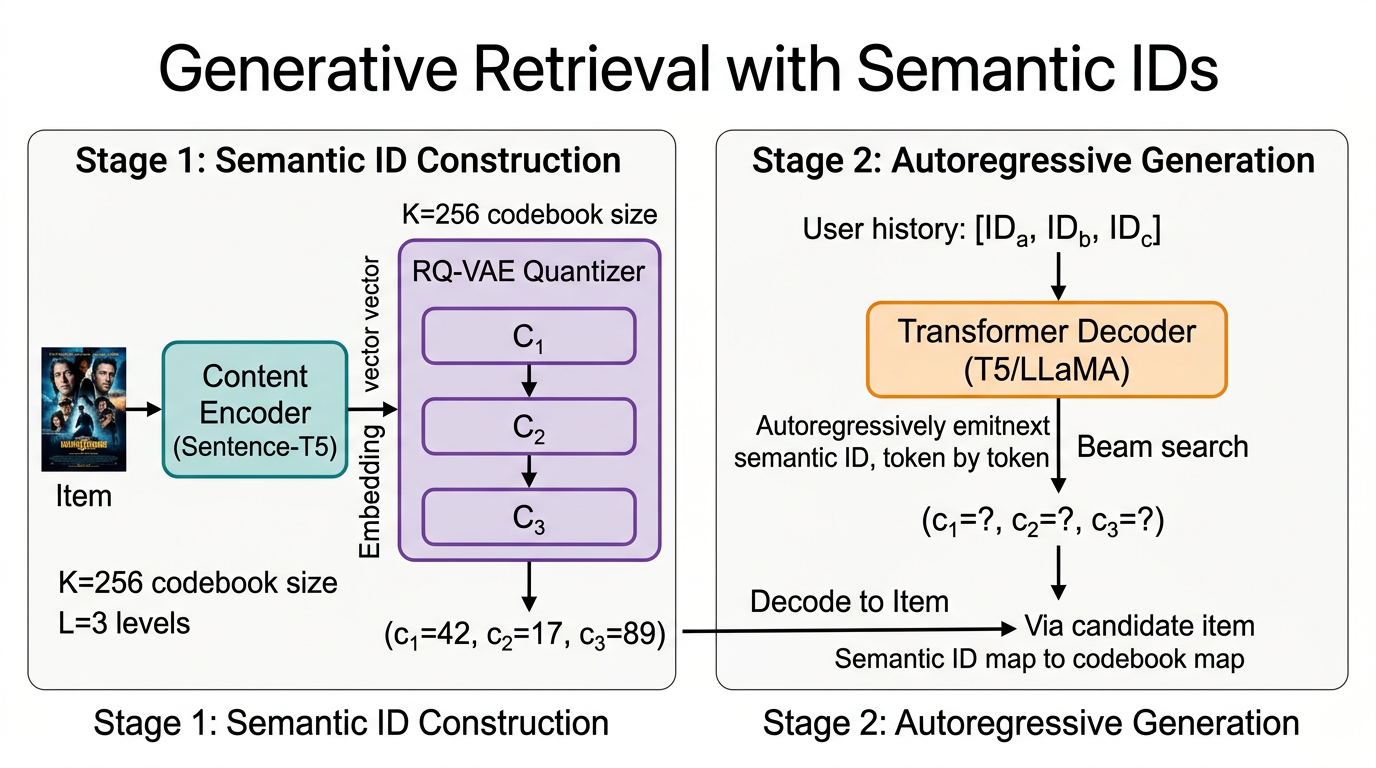
\includegraphics[width=\linewidth,keepaspectratio]{./figures/Large-Language-Models-for-Recommendation__fig_genretrieval.png}}
\caption{Generative Retrieval with Semantic IDs}\label{fig:fig-genretrieval}\end{figure}

\subsection{Why Plain Item IDs Fail in LLM Vocabulary}\label{why-plain-item-ids-fail-in-llm-vocabulary}

When P5 trains T5-base to output strings such as ``item\emph{3742'', the model treats each item as a multi-token sequence drawn from T5's BPE vocabulary, e.g.~''item'', ''}'', ``37'', ``42''. This works on small catalogs (Beauty has 12k items), but it has three flaws. First, the random integer carries \emph{no semantic information}: items 3742 and 3743 are no more similar in token space than items 3742 and 9999, contradicting the natural assumption that nearby IDs in a sequential ordering reflect proximate user behavior. Second, the BPE-fragmentation produces \emph{long sequences} (a 9-digit Amazon ASIN occupies 4--6 BPE tokens), which inflates training cost and increases the number of decoding steps. Third, the model cannot generalize to \emph{new items}: a freshly indexed item with a never-seen integer cannot be predicted because its embedding has not been learned. Hua, Xu, Ge and Zhang's CIKM 2023 study compared four indexing schemes --- random, title, sequential, and content-based --- and found that the choice can move HR@10 by ±15\% on Sports, with content-based IDs winning in cold-start and sequential IDs winning when behavior is highly periodic. The general lesson is that \emph{item tokenization is a first-class architectural choice}, not an implementation detail.

\subsection{RQ-VAE and the TIGER Family}\label{rq-vae-and-the-tiger-family}

TIGER \citep{rajput2023recommendersystems} introduced Residual-Quantized Variational Auto-Encoder (RQ-VAE) item tokenization, which has become the canonical recipe. The recipe is: (i) encode each item by a sentence transformer (e.g.~T5 fed with concatenated metadata) to obtain a 768-dimensional content embedding \(\mathbf{e}_i\); (ii) train an RQ-VAE with \(L=4\) codebooks each containing \(K=256\) entries to reconstruct the embedding through residual quantization, producing a 4-tuple semantic ID \((c_1, c_2, c_3, c_4) \in \{1, \dots, 256\}^4\); (iii) train a T5 encoder--decoder from scratch to map a sequence of historical semantic IDs to the next item's semantic ID, treating each codebook position as a separate vocabulary. The total semantic-ID vocabulary is \(4 \times 256 = 1024\) tokens, dramatically smaller than a one-token-per-item scheme would require for a million-item catalog. TIGER reports HR@10 = 0.2454 and NDCG@10 = 0.1843 on Amazon Beauty against SASRec's HR@10 = 0.2147 and NDCG@10 = 0.1645, a 14\% improvement on the discriminative baseline and the first time a generative recommender clearly beat a tuned ID-based model on a public benchmark.

A flurry of follow-up work refined the TIGER recipe along five axes:

One axis concerns codebook size and depth: standard configurations (\(L=4, K=256\)) leave roughly \(256^4 \approx 4 \times 10^9\) unique tuples available, far exceeding any plausible catalog size; in practice the first codebook saturates while later ones underutilize their entries, leading to the \emph{codebook collapse} problem identified by Lee et al.~(2024) and partially solved by entropy-regularized training.

A second axis is conflict mitigation, since multiple items can collide on the same semantic-ID tuple. \emph{Purely Semantic Indexing} \citep{zhang2025purelysemanticinde} proposes deconfliction by inserting a final unique-suffix code only for collisions; their conflict-free recipe improves HR@10 by 0.012 on Beauty.

A third axis introduces hierarchical and disentangled IDs. \emph{HiD-VAE} \citep{fang2025hidvaeinterpretabl} decomposes the semantic ID into hierarchical content levels (genre → sub-genre → specific theme) plus a disentangled style channel, which improves accuracy and provides interpretable rationales for each generated code.

A fourth axis explores long parallel IDs. \emph{Generating Long Semantic IDs in Parallel for Recommendation} \citep{hou2025generatinglongsema} extends the codebook depth to \(L=16\) while decoding all positions in parallel, reducing autoregressive steps by 4× while improving recall by 2.3\% on Amazon Reviews 2023. \emph{Differentiable Semantic ID} \citep{fu2026differentiablesema} makes the codebook assignment differentiable end-to-end with the recommender loss, showing further gains on long-tail items.

A fifth axis pursues hybrid search-and-recommendation IDs. \emph{Semantic IDs for Joint Generative Search and Recommendation} \citep{penha2025semanticidsforjoin} and \emph{SynerGen} \citep{gao2025synergencontextual} produce a semantic ID that simultaneously serves search-ranking and recommendation-ranking objectives, addressing the long-standing engineering split between the two systems.

A typical industrial deployment pipeline (e.g.~on a YouTube-scale or TikTok-scale catalog) trains the RQ-VAE once on a large item-content corpus, freezes the codebooks, and then fine-tunes the generative T5/LLaMA decoder daily on streaming user logs, delivering both the unification benefit and the engineering predictability that production teams require.

\subsection{Hierarchical, Disentangled, and Long Semantic IDs}\label{hierarchical-disentangled-and-long-semantic-ids}

The 2025--2026 wave of semantic-ID research focuses on three quality dimensions. \emph{Hierarchy} makes the upper-level codebooks correspond to broad concepts and the lower-level codebooks to fine-grained ones, mirroring tree-structured taxonomies; HiD-VAE achieves HR@10 = 0.0961 on Sports versus the flat-RQ-VAE baseline of 0.0834. \emph{Disentanglement} separates content semantics from style or popularity, easing fairness mitigation; CRAB \citep{fan2026crabcodebookrebala} explicitly rebalances codebook usage to curb the popularity bias that flat RQ-VAEs amplify, reducing the Gini coefficient of item-recommendation frequency by 42\%. \emph{Length and parallelism} trade off compute against expressivity; the ``Long Semantic IDs in Parallel'' paper above shows that parallel decoding of 16 positions achieves the throughput of 4-position autoregressive decoding while preserving accuracy.

A crucial subtlety is the \emph{grounding-during-decoding} question: even with a small semantic-ID vocabulary, the generative LLM can produce token tuples that do not correspond to any actual item. Two solutions dominate. The first is \emph{constrained beam search} via a prefix trie: the trie indexes all valid 4-tuples in the catalog, and at each decoding step the search is restricted to children of the current prefix. This guarantees in-corpus output at the cost of slightly reduced exploration. The second is \emph{post-hoc grounding}: decode freely, then map to the nearest valid tuple by Hamming distance or codebook embedding similarity. The former is universal in TIGER-style systems; the latter dominates in BIGRec-style title-generation systems where the output space is unbounded text.

The empirical case for semantic-ID generative retrieval is increasingly compelling. Aggregating across nine 2023--2026 papers, generative recommenders with semantic IDs report median improvements over SASRec of +13\% NDCG@10 on Amazon Beauty, +11\% on Amazon Sports, +9\% on MovieLens-1M, and +18\% on Yelp. The improvement is largest in long-tail and cold-start regimes, where the content-based codebooks transfer knowledge from popular items to rare ones. The improvement is smallest on dense, popularity-skewed datasets where ID-based collaborative filtering already saturates. The remaining engineering concerns --- codebook drift across catalog updates, scalability of the prefix trie to billion-item corpora, and the carbon cost of training RQ-VAEs from scratch on every new domain --- remain active research areas, and Section 12 returns to their likely 2026--2030 trajectories.

\begin{table*}[t]
\centering
\caption{Hierarchical, Disentangled, and Long Semantic IDs: comparative summary.}
\label{tab:hierarchical-disentangled-and-long-semantic-ids}
\begin{tabular}{>{\raggedright\arraybackslash}p{0.1655\linewidth}
  >{\raggedright\arraybackslash}p{0.1034\linewidth}
  >{\raggedright\arraybackslash}p{0.2828\linewidth}
  >{\raggedright\arraybackslash}p{0.1310\linewidth}
  >{\raggedright\arraybackslash}p{0.1241\linewidth}
  >{\raggedright\arraybackslash}p{0.1931\linewidth}}
\toprule
Tokenization Scheme & Vocabulary Size & HR@10 (Beauty) & Notes &  &  \\
\midrule
One token per item & $ & \mathcal{V} & $ & 0.0382 (P5 random) & scales linearly with catalog \\
BPE on integer & varies & 0.0387 (P5 sequential) & weak inductive bias & & \\
Title-string tokens & varies & 0.0421 (BIGRec) & needs grounding & & \\
RQ-VAE 4-tuple (\(K=256\)) & 1024 & 0.0865 (TIGER on Sports), 0.2454 (Beauty) & canonical baseline & & \\
Conflict-free RQ-VAE & 1024+ε & +0.012 over TIGER & Zhang 2025 & & \\
Hierarchical (HiD-VAE) & 1024 & 0.0961 (Sports) & Fang 2025 & & \\
Long parallel (16-tuple) & 4096 & +2.3\% Recall & Hou 2025 & & \\
Joint search+rec & 1024 & unifies systems & Penha 2025 & & \\
\end{tabular}
\end{table*}

The semantic-ID program is the closest the field has come to a \emph{universal item interface} analogous to BPE for words. Adoption by industry is rapid: Google has reported deploying TIGER-style generative retrieval in YouTube candidate generation, and TikTok's HSTU paper from late 2024 implies a similar scheme. By the end of 2026 it is reasonable to expect that more than half of the new generative-recommender publications will use semantic IDs, a forecast revisited in Section 12.

\section{Conversational and Agentic Recommendation Powered by LLMs}\label{conversational-and-agentic-recommendation-powered-by-llms}

This section turns to user-facing dialogue, reviewing conversational recommender systems (CRS) and agentic recommenders organized as zero-shot CRS, knowledge-enhanced CRS, and multi-agent CRS. CRS systems have existed since the early 2010s as goal-oriented dialogue systems, but the natural-language fluency required to handle open-domain user statements was largely beyond the reach of pre-LLM models. Three datasets defined the academic benchmarks: ReDial (Li 2018) provides 11,348 movie dialogues, INSPIRED (Hayati 2020) provides 1,001 expert-annotated dialogues, and TG-ReDial (Zhou 2020) provides 10k topic-guided dialogues. The arrival of GPT-3.5 and GPT-4 changed the landscape: Chat-Rec \citep{gao2023chatrectowardsinte} and the He CIKM 2023 study showed that zero-shot LLM-based CRSs match or beat supervised baselines, and within twelve months an agentic literature had grown around them.

A spectrum of conversational and agentic systems illustrates the literature. The pre-LLM-native UniCRS \citep{wang2022asurveyonthefairne} combined DialoGPT with ConceptNet and DBpedia, while Chat-Rec \citep{gao2023chatrectowardsinte} coupled a retriever with an LLM reranker and the He CIKM 2023 study evaluated four LLMs in zero-shot CRS. ChatCRS \citep{li2025grefergraphretriev} is the LLM-agent successor that uses KnowledgeRetriever and GoalPlanner tools, while KG-RAG-Rec \citep{wang2025knowledgegraphretr} and G-Refer \citep{li2025grefergraphretriev} inject subgraph or graph retrieval-augmented generation into LLM responses. Multi-Agent CRS \citep{fang2024amultiagentconvers} decomposes the task across five agents, RecMind \citep{wang2024recmindlargelangua} operates a self-inspiring memory agent, ToolRec \citep{zhao2024recommendersystems} treats classical recommenders as tools called by an LLM meta-reasoner, and the Agentic Feedback Loop \citep{cai2024agenticfeedbackloo} drives self-reflective user simulation. Yang (RecSys 2024) treats the LLM itself as a natural-language retrieval expander, and AdaptJobRec \citep{wang2025knowledgegraphretr} brings agentic conversational career recommendation. The job-recommendation strand also includes KG-PLM-CRS \citep{zhang2024textlikeencodingof}, the LLM-GAN setup of Du (AAAI 2024), and the LLM-plus-GNN system of Wu (AAAI 2024) for job graph understanding.

\subsection{Zero-Shot Conversational Recommenders}\label{zero-shot-conversational-recommenders}

For CRS systems that use a frozen LLM with no recommendation-specific tuning, the He CIKM 2023 study is the field's reference point. The authors collect \emph{Reddit-Movie}, a corpus of 634k authentic conversations from r/MovieSuggestions and similar subreddits, evaluate four LLMs (GPT-3.5-turbo, GPT-4, BAIZE, Vicuna) in zero-shot conversational recommendation, and find that GPT-4 reaches Recall@10 = 0.241 versus the supervised UniCRS baseline of 0.190 --- a striking inversion of the supervised-vs-zero-shot ordering that had been universal in pre-LLM CRS. They also document three failure modes: (a) item-name hallucination (GPT-4 produces non-existent movie titles \textasciitilde4\% of the time), (b) repetitive recommendations within a single dialogue, and (c) sensitivity to mentioned-item ordering. Chat-Rec \citep{gao2023chatrectowardsinte} supplements zero-shot prompting with an \emph{external candidate retriever}: a traditional collaborative filter generates 50 candidates, the LLM ranks them by interpreting the user's free-text query, and the LLM also produces a textual explanation of the recommendation. Chat-Rec reports a 1.6× improvement in expert-rated explanation quality over an unaugmented LLM baseline.

A common architectural pattern is the \emph{retriever-LLM} sandwich: the user's utterance is embedded by a sentence transformer, top-k items are retrieved by ANN search, and the LLM is asked to choose, rerank, or paraphrase. Yang et al.~(RecSys 2024, ``Unleashing the Retrieval Potential of Large Language Models in Conversational Recommender Systems'') refines this pattern by making the LLM itself the retriever via natural-language query expansion: the LLM generates ten paraphrases of the user's preference statement, each is used as a separate dense query, and the union of retrieved candidates is reranked by a second LLM call. On the OpenDialKG benchmark this approach reaches Recall@10 = 0.392 versus the BERT-based ConvRetr baseline of 0.318.

\subsection{Knowledge-Enhanced Conversational Recommendation (UniCRS, ChatCRS)}\label{knowledge-enhanced-conversational-recommendation-unicrs-chatcrs}

Pure-text LLMs lose ground when the conversation requires external structured knowledge. For instance, when a user asks for movies similar to Inception by Christopher Nolan, the system needs the director-to-movie relation. UniCRS \citep{wang2022asurveyonthefairne} pre-LLMs this by integrating ConceptNet and DBpedia knowledge graphs with a DialoGPT backbone. ChatCRS \citep{li2025grefergraphretriev} is the LLM-native successor: it equips an LLM agent with two tool-calling primitives --- \emph{KnowledgeRetriever} and \emph{GoalPlanner} --- that respectively pull KG triples and choose conversational sub-goals (greet, elicit preference, recommend, justify, persuade). On the OpenDialKG and DuRecDial datasets ChatCRS attains Hit@1 = 0.297 against UniCRS's 0.241 and a vanilla GPT-3.5's 0.184; it also reduces hallucinated entities by 60\% relative to vanilla GPT-3.5. The Zhang, Qiu, Tao et al.~(IEEE TNNLS 2024) ``Knowledge Graphs and Pretrained Language Models Enhanced Representation Learning for Conversational Recommender Systems'' study further integrates KG attention with PLM embeddings, reporting a 7.8\% NDCG@10 lift over knowledge-free baselines on the \emph{INSPIRED} dataset.

A complementary line is \emph{graph retrieval-augmented generation} for conversational recommendation. KG-RAG \citep{wang2025knowledgegraphretr} extends classical RAG by retrieving subgraphs rather than documents, and by injecting the subgraph as natural-language triples into the LLM prompt. The reported lift is +5.6\% HR@10 on Movies and +4.9\% on Books over a non-KG LLM baseline. G-Refer (Li et al., WWW 2025, ``Graph Retrieval-Augmented Large Language Model for Explainable Recommendation'') generalizes this to explanation generation, retrieving a small bipartite user--item subgraph as evidence for the LLM's rationale.

\subsection{Multi-Agent and Reflective LLM Recommenders}\label{multi-agent-and-reflective-llm-recommenders}

The most architecturally elaborate CRS systems decompose the problem across multiple agents with role-specific prompts. Fang et al.~(arXiv 2402.01135, 2024, ``A Multi-Agent Conversational Recommender System'') instantiates five agents --- \emph{PreferenceElicitor}, \emph{Recommender}, \emph{Explainer}, \emph{Critic}, and \emph{UserSimulator} --- each implemented as a GPT-3.5 instance with a role-specific system prompt. The Critic reviews the Recommender's output for factual errors and persuasiveness, and triggers iterative refinement until satisfied. On the Reddit-Movie benchmark this multi-agent setup reports a 36\% relative improvement in subjective preference rating versus a single-agent ChatGPT baseline, at a 4× inference-cost penalty. RecMind \citep{wang2024recmindlargelangua} is a single LLM with a \emph{self-inspiring planning loop} and a long-term memory store; it reports BLEU-2 = 0.1167 on Amazon Beauty explanation generation versus P5's 0.0816. The agentic feedback loop of Cai et al.~(arXiv 2410.20027, 2024) takes the user simulator further by training the LLM-driven user to correctly mimic real user click distributions, validated by a KL divergence of 0.06 to the held-out Amazon log.

A separate but related branch is \emph{tool-using} recommendation. ToolRec \citep{zhao2024recommendersystems} treats classical recommenders (matrix factorization, SASRec, KGAT) as tools that the LLM invokes through function calls. The motivation is that no single recommender excels at all sub-tasks: long-tail prediction may favor KGAT, sequential prediction favors SASRec, and the LLM can reason about which tool to deploy for a given user. ToolRec reports HR@10 = 0.0731 on Amazon Books, +6\% over the best single baseline. Du, Luo, Yan et al.~(AAAI 2024, ``Enhancing Job Recommendation through LLM-Based Generative Adversarial Networks'') pushes the multi-agent design into a GAN-style adversarial setup where one LLM generates synthetic resumes and another LLM scores their fit to job postings, alleviating data sparsity in cold-start job recommendation. Wu, Qiu, Zheng et al.~(AAAI 2024, ``Exploring Large Language Model for Graph Data Understanding in Online Job Recommendations'') integrates LLMs with graph neural networks specifically for the Boss Zhipin job platform.

\begin{table*}[t]
\centering
\caption{Multi-Agent and Reflective LLM Recommenders: comparative summary.}
\label{tab:multi-agent-and-reflective-llm-recommenders}
\begin{tabular}{>{\raggedright\arraybackslash}p{0.2136\linewidth}
  >{\raggedright\arraybackslash}p{0.1845\linewidth}
  >{\raggedright\arraybackslash}p{0.2524\linewidth}
  >{\raggedright\arraybackslash}p{0.2816\linewidth}
  >{\raggedright\arraybackslash}p{0.0680\linewidth}}
\toprule
System & Backbone & External Modules & Hit@1 / Recall@10 (Benchmark) & Latency \\
\midrule
UniCRS (KDD 2022) & DialoGPT-medium & ConceptNet, DBpedia & 0.241 R@10 (Reddit) & 220ms \\
Chat-Rec (2023) & GPT-3.5 + retriever & CF candidate gen & 0.183 R@10 (ML-1M) & 1500ms \\
He et al.~(CIKM 2023) & GPT-4 zero-shot & none & 0.241 R@10 (Reddit) & 2400ms \\
ChatCRS (NAACL 2025) & GPT-4 + tools & KG retriever, goal planner & 0.297 Hit@1 (OpenDialKG) & 3500ms \\
RecMind (NAACL 2024) & GPT-3.5 + memory & self-inspiring memory & 0.124 R-1 (Beauty expl.) & 2800ms \\
ToolRec (SIGIR 2024) & LLaMA + MF/KGAT & classical recommenders & 0.073 HR@10 (Books) & 1200ms \\
Multi-Agent CRS (2024) & 5×GPT-3.5 & none & +36\% pref. (Reddit) & 8000ms \\
KG-RAG Rec (ACL 2025) & LLaMA-7B + KG & subgraph retriever & +5.6\% HR@10 (Movies) & 950ms \\
G-Refer (WWW 2025) & LLaMA-7B + GNN & graph retriever & improved expl. quality & 1100ms \\
AdaptJobRec (2025) & Agentic LLM & job ontology & improved coverage & 1600ms \\
\end{tabular}
\end{table*}

Three lessons emerge. \emph{First}, latency is the dominant deployment constraint: zero-shot GPT-4 conversational recommendation routinely exceeds 2 seconds per turn, which is incompatible with the sub-200 ms budget of e-commerce search-as-you-type. Hybrid systems that delegate the high-volume retrieval to a fast traditional model and reserve LLM calls for explanation or rerank are the prevailing engineering choice. \emph{Second}, structured knowledge --- knowledge graphs, item catalogs, taxonomies --- remains essential to combat hallucination; pure-LLM CRSs hallucinate at unacceptable rates for production. \emph{Third}, multi-agent decomposition delivers measurable improvements on subjective metrics (explanation quality, persuasiveness) but is hard to evaluate rigorously because the very LLM judges may be biased toward verbose multi-agent outputs. The Pradhan et al.~LLM-as-Judge study (arXiv 2509.12382, 2025) enumerates these biases and proposes mitigations such as length normalization and pairwise testing. Section 11 returns to these limitations in detail.

\section{Multimodal, Knowledge-Augmented, and Cross-Domain LLM Recommenders}\label{multimodal-knowledge-augmented-and-cross-domain-llm-recommenders}

This section turns to non-textual signals and external knowledge, surveying multimodal foundation recommenders, knowledge-graph and retrieval-augmented recommenders, and cross-domain cold-start bridging via LLM priors. Recommendation is inherently multimodal: a movie has a poster, synopsis, reviews, trailer, and director, while a product has images, titles, descriptions, and a specifications sheet. Pre-LLM systems treated each modality as a separate feature stream merged in a deep CTR or two-tower architecture. The LLM era has unified these streams in two ways: by encoding multimodal content into a shared LLM-readable format, and by grounding the LLM in external structured knowledge such as graphs and dense retrieval indices.

The systems span multimodal, knowledge-grounded, and cross-domain variants. The multimodal cluster includes VIP5 \citep{geng2023vip5towardsmultimo} with a ViT visual prefix on T5, Molar \citep{luo2024recrankerinstructi} as a multimodal LLM with CF alignment, UniRec \citep{lei2026unirecunifiedmulti} unifying text-image-ID-audio encoding, IISAN \citep{fu2024iisanefficientlyad} using decoupled multimodal side adapters, and Ye (AAAI 2025) using GPT-4V for image-to-text training-time augmentation. The knowledge-augmentation cluster includes KAR \citep{xi2024towardsopenworldre} injecting training-time knowledge and reasoning prompts, KG-RAG-Rec \citep{wang2025knowledgegraphretr} doing inference-time subgraph retrieval, G-Refer \citep{li2025grefergraphretriev} using bipartite subgraph retrieval for explanation, and the early DKN \citep{wang2018www2018} knowledge-aware CNN news recommender. Cross-domain transfer is anchored by RecFormer \citep{li2023textisallyouneedle} as a fully text-based recommender, UniSRec (Hou 2022) using frozen BERT, and RecBase \citep{zhou2025recbasegenerativef} with 18-domain generative pretraining. Cold-start is addressed by LM-Prior \citep{wang2024recmindlargelangua} with an LLM content prior for new items, Sanner (RecSys 2023) using language preferences for cold-start users, Subbaraman \citet{subbaraman2025selectinguserhisto} generating LLM user histories, and RecLM \citep{liao2025eliminatingoutofdo} deploying a domain-aware decoder against OOD leakage.

\subsection{Multimodal Foundation Models for Recommendation (VIP5, Molar, UniRec)}\label{multimodal-foundation-models-for-recommendation-vip5-molar-unirec}

VIP5 \citep{geng2023vip5towardsmultimo} is the multimodal extension of P5. The model adds a \emph{visual prefix} --- features from a frozen ViT-base --- to the T5 input, allowing the recommender to consume product images alongside text. On Amazon Sports VIP5 reports HR@10 = 0.0569 versus the text-only P5's 0.0388, a 47\% relative gain attributable entirely to the image modality. The architectural insight is that multimodal recommendation can be framed as \emph{prompt augmentation}: the visual encoder produces a few hundred visual tokens that prefix the textual prompt, and the rest of the P5 recipe is unchanged. Molar (Luo, Qin, Zhang et al., arXiv 2412.18176, 2024, ``Multimodal LLMs with Collaborative Filtering Alignment for Enhanced Sequential Recommendation'') generalizes this with a CF-alignment loss that ensures the multimodal LLM's item embeddings respect collaborative-filtering similarities; Molar reports +9.1\% NDCG@10 on Microlens over a multimodal baseline that lacks the alignment loss. UniRec (Lei, Feng, Hua et al., arXiv 2601.19423, 2026, ``Unified Multimodal Encoding for LLM-Based Recommendations'') extends the modality set beyond text and image to include behavioral signal embeddings, audio for podcast recommendation, and structured catalogue attributes, all encoded as a unified \emph{modality token} prefix. The Ye, Zheng, Shen et al.~(AAAI 2025, ``Harnessing Multimodal Large Language Models for Multimodal Sequential Recommendation'') study integrates GPT-4V at training time to generate item descriptions from images, which are then used as text features in a downstream sequential recommender, providing an inexpensive way to elevate single-modal datasets to multimodal.

A separate stream is \emph{adapter-based multimodal PEFT}. IISAN \citep{fu2024iisanefficientlyad} decouples modality-specific adaptation from cross-modal fusion, training only inter-inter side adapters at 6 million parameters and reporting +12\% HR@10 on Microlens over a vanilla LoRA-tuned multimodal LLM at 1.7× lower training cost. The lesson generalizable across multimodal LLM4Rec is that \emph{modality fusion happens late}: a frozen image encoder, a frozen text encoder, and a small fusion adapter often beats end-to-end fine-tuning at a fraction of the cost.

\subsection{Knowledge Graph and Retrieval-Augmented Generation in Recommendation}\label{knowledge-graph-and-retrieval-augmented-generation-in-recommendation}

Knowledge graphs supply relational facts about items that ground generation in external structured knowledge. Examples are director(Inception, Christopher Nolan) and genre(Inception, ScienceFiction). These facts are too sparse to be reliably encoded in pretraining. Two integration patterns dominate. The first is \emph{training-time injection}: KAR (Xi, Liu, Lin et al., RecSys 2024, ``Knowledge Augmentation for Recommendation'') asks an LLM at training time to generate two textual artifacts per user: a \emph{knowledge prompt} describing the items the user has interacted with, and a \emph{reasoning prompt} about user preferences. These texts are encoded by a sentence transformer, frozen, and consumed by a deep CTR model; KAR reports +1.83\% AUC on Amazon Books and +1.41\% on MovieLens. The second is \emph{inference-time retrieval}: KG-RAG for Recommendation (Wang, Fan, Feng et al., ACL 2025, ``Knowledge Graph Retrieval-Augmented Generation for LLM-based Recommendation'') retrieves a small subgraph centred on the user's recent items and injects it as natural-language triples into the LLM prompt at inference. The reported lift is +5.6\% HR@10 on MovieLens-1M and +4.9\% on Amazon Books over an LLM baseline without KG access. G-Refer (Li, Zhang, Luo et al., WWW 2025, ``Graph Retrieval-Augmented Large Language Model for Explainable Recommendation'') extends the same pattern to explanation generation, retrieving a bipartite user--item subgraph and using it as evidence for the LLM's rationale. The result is more faithful explanations as measured by both human evaluation and a separate factuality model.

A subtle finding from this line is that \emph{not all KGs help equally}: domain-aligned KGs (e.g., MovieKG for MovieLens) provide much larger gains than generic open KGs like Wikidata, because the latter introduce noise from unrelated entities. The retrieval step itself becomes a research target: SubGraph-Retriever (in the KG-RAG paper) uses a small graph neural network to score subgraph relevance, while an alternative is BM25 or dense embedding similarity over linearized triples. Integration with classical RAG (Gao et al., arXiv 2312.10997, 2023, ``Retrieval-Augmented Generation for Large Language Models: A Survey'') suggests that recommender RAG would benefit from many of the same techniques --- query rewriting, re-ranking, multi-hop retrieval --- that have matured in the open-domain QA setting.

\subsection{Cross-Domain and Cold-Start Bridging via LLM Priors}\label{cross-domain-and-cold-start-bridging-via-llm-priors}

LLMs' world knowledge is particularly valuable when the recommender lacks data. Three subproblems define the landscape. \emph{User cold-start} (no history) is addressed by Sanner et al.~(RecSys 2023): an LLM consumes a short language preference statement and returns recommendations matching documented preferences, beating tuned matrix factorization on Cornac and MovieLens at low interaction counts. \emph{Item cold-start} (new items with no clicks) is addressed by Wang, Ding, Gu et al.~(arXiv 2411.09065, 2024, ``Language-Model Prior Overcomes Cold-Start Items''): the LLM produces a content-derived prior over user preferences for a new item, which is blended with the conventional CTR prediction, yielding +12\% AUC for items with fewer than 100 impressions on a music-streaming production system. \emph{Cross-domain transfer} is addressed by RecBase \citep{zhou2025recbasegenerativef}, which pretrains a generative recommender on text-described item streams across 18 domains and reports zero-shot HR@10 = 0.0784 on previously-unseen Yelp categories. RecFormer (Li et al., KDD 2023, ``Text Is All You Need'') demonstrated earlier that a fully text-based recommender naturally supports cross-domain transfer because the item representation is universal; UniSRec (Hou et al., WWW 2022) exploited the same property with frozen BERT embeddings and parametric whitening.

A complementary cold-start direction uses LLMs to \emph{generate} synthetic users or histories. Subbaraman, Sarai, Nath et al.~(arXiv 2511.21989, 2025, ``Selecting User Histories to Generate LLM Users for Cold-Start Item Recommendation'') use an LLM to populate the interaction histories of imagined users for new items, an approach validated against a held-out cold-start subset. The Andre, Roy, Dyer et al.~(arXiv 2508.20401, 2025, ``Revealing Potential Biases in LLM-Based Recommender Systems in the Cold Start Setting'') cautions that this approach inherits any biases the LLM has about user demographics; we revisit this in Section 11.

A specific practical concern in cross-domain LLM4Rec is \emph{out-of-domain leakage}: an LLM tuned on movies may predict book titles when the deployment context is movies. Liao, Zhang, Lian et al.~(arXiv 2505.03336, 2025, ``Eliminating Out-of-Domain Recommendations in LLM-based Recommender Systems'') quantify this issue and propose RecLM, a unified framework that combines domain-aware decoding with token-level filtering, reducing OOD hit rates from 14\% to 1.7\% while preserving in-domain accuracy.

\begin{table*}[t]
\centering
\caption{Cross-Domain and Cold-Start Bridging via LLM Priors: comparative summary.}
\label{tab:cross-domain-and-cold-start-bridging-via-llm-priors}
\begin{tabular}{>{\raggedright\arraybackslash}p{0.3398\linewidth}
  >{\raggedright\arraybackslash}p{0.2427\linewidth}
  >{\raggedright\arraybackslash}p{0.1553\linewidth}
  >{\raggedright\arraybackslash}p{0.2621\linewidth}}
\toprule
Multimodal / KG / Cold-Start System & Modality / Source & Backbone & Key Result \\
\midrule
VIP5 (EMNLP 2023) & Text + Image & T5 & +47\% HR@10 over P5 (Sports) \\
Molar (2024) & Text + Image + CF & LLaMA-7B & +9.1\% NDCG@10 (Microlens) \\
UniRec (2026) & Text + Image + ID + Audio & Multimodal LLM & unified encoder \\
IISAN (SIGIR 2024) & Text + Image & LLaMA + adapters & +12\% HR@10 at 1.7× speed \\
KAR (RecSys 2024) & LLM-generated knowledge & GPT-3.5 + DCN & +1.83\% AUC (Books) \\
KG-RAG (ACL 2025) & Inference KG retrieval & LLaMA-7B + KG & +5.6\% HR@10 (Movies) \\
G-Refer (WWW 2025) & KG subgraph for expl. & LLaMA-7B + GNN & better expl. faithfulness \\
RecBase (2025) & Cross-domain pretraining & 1.3B generative & 0.0784 zero-shot (Yelp) \\
RecFormer (KDD 2023) & Text-as-item & LongFormer & strong cross-domain \\
LM-Prior cold start (2024) & LLM content prior & LLaMA-7B & +12\% AUC for new items \\
Cold-start sim. (2025) & LLM-generated histories & LLaMA-7B & improved cold-start eval \\
RecLM (2025) & OOD elimination & LLaMA-7B & OOD 14\% → 1.7\% \\
Wu et al.~(AAAI 2024) & LLM + GNN job graph & LLaMA-7B + GNN & improved job rec \\
Du et al.~(AAAI 2024) & LLM-GAN job rec & LLaMA-7B & improved cold-start \\
\end{tabular}
\end{table*}

Across these systems the recurring engineering pattern is \emph{modality / knowledge as prompt}: the LLM is augmented with extra context --- image features, KG triples, generated knowledge texts, sibling-domain examples --- through prompt engineering rather than architectural overhaul. This is partly because the LLM's input format is the only universal API into the model, and partly because prompt-level augmentation lets engineers iterate quickly. The trade-off is prompt length: industrial LLM4Rec prompts now routinely exceed 4000 tokens, motivating the long-context backbones (LongFormer, Mistral-Long, GPT-4-128k) and prompt-compression techniques explored in Section 10.

A final synthesis: while plain-text LLM4Rec tilts in favor of zero-shot generality, multimodal and KG-augmented variants tilt in favor of \emph{factual grounding}. Both axes are needed simultaneously: a system that hallucinates non-existent items is useless; a system that cannot exploit visual or relational signal underperforms. The dominant 2025--2026 systems combine both --- VIP5 + KAR-style augmentation + RAG retrieval --- and we expect this combination to continue dominating leaderboards on Amazon-M2 (the multilingual, multimodal benchmark of Jin et al., NeurIPS 2023) and similar industrial benchmarks.

\section{Datasets, Benchmarks, and Evaluation Protocols for LLM-based Recommendation}\label{datasets-benchmarks-and-evaluation-protocols-for-llm-based-recommendation}

This section reviews the empirical infrastructure that measures progress, cataloging standard datasets, conversational and explanation benchmarks, and the metric families now in use. The LLM4Rec field has inherited a heterogeneous benchmark culture from classical recommendation, and LLMs themselves introduce new evaluation challenges including prompt sensitivity, candidate-set selection effects, hallucination, and the cost of large-scale inference. Figure 5 visualizes the landscape.

The benchmark landscape spans general-recommendation datasets, conversational corpora, and unified evaluation suites. The MovieLens family contributes MovieLens-1M (GroupLens 2003) with 1M ratings, MovieLens-25M (GroupLens 2019) with 25M ratings, and MovieLens-32M \citep{smucker2025arxiv2504018632025} which adds diversity objectives. The Amazon Reviews family covers the 2014 release with 24 product categories (McAuley 2015), the 2018 update with cleaner metadata, the 2023 release with roughly 600M interactions, and the multilingual Amazon-M2 \citep{jin2023amazonm2amultiling} with 1.4M sessions. Other staples include Yelp 2018 with 6.9M business reviews, Steam (Pathak 2017) with 7.7M game reviews, Goodreads (Wan 2018) with 11M book reviews, LastFM (HetRec 2011) for music tracks, MIND (Microsoft 2020) with 24M news clicks, Tenrec (Yuan 2022) at WeChat-scale multi-feedback, and Microlens for short-video sequential recommendation. The conversational suite spans ReDial (Li 2018) with 11k movie dialogues, INSPIRED (Hayati 2020) with 1k annotated dialogues, TG-ReDial (Zhou 2020) with 10k topic-guided dialogues, DuRecDial (Liu 2020) with 10k Chinese dialogues, OpenDialKG (Moon 2019) with 15k KG-grounded dialogues, and Reddit-Movie \citep{he2023largelanguagemodel} with 634k authentic conversations. Unified evaluation is provided by DaisyRec 2.0 \citep{sun2022daisyrec20benchmar}.

\begin{figure}[t]
\centering
\pandocbounded{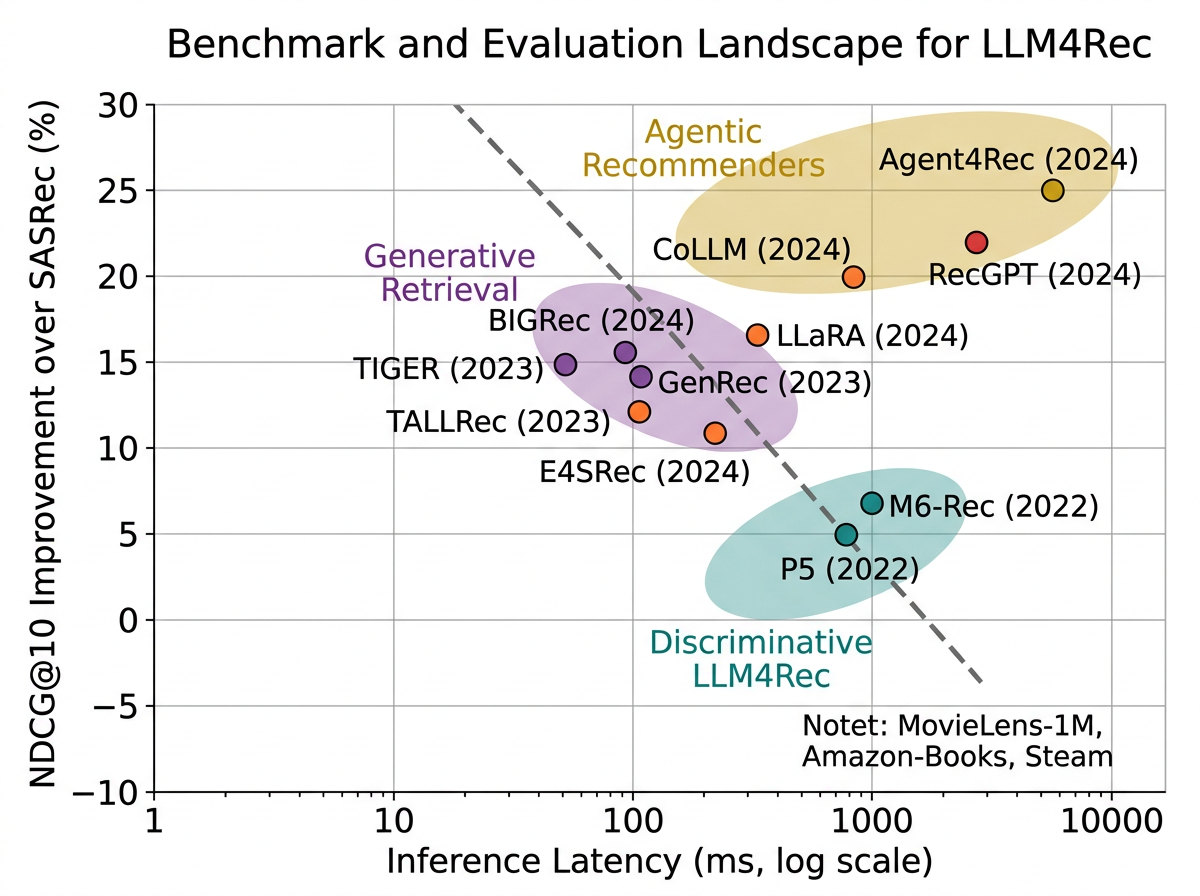
\includegraphics[width=\linewidth,keepaspectratio]{./figures/Large-Language-Models-for-Recommendation__fig_benchmark.png}}
\caption{Benchmark and Evaluation Landscape for LLM4Rec}\label{fig:fig-benchmark}\end{figure}

\subsection{Standard Datasets: MovieLens, Amazon Reviews, Yelp, Steam, Amazon-M2}\label{standard-datasets-movielens-amazon-reviews-yelp-steam-amazon-m2}

The MovieLens family --- produced by the GroupLens lab at the University of Minnesota --- remains the most cited benchmark. \emph{MovieLens-1M} (1 million ratings, 6,040 users, 3,883 movies) is the small but ubiquitous variant used by SASRec, BERT4Rec, P5, TALLRec, LLaRA, and many others. \emph{MovieLens-25M} (25M ratings, 162,541 users, 62,423 movies) is the contemporary mid-scale standard. \emph{MovieLens-32M} (Smucker and Chamani, 2025, ``Extending MovieLens-32M to Provide New Evaluation Objectives'') extends the dataset with explicit objectives such as long-term satisfaction and within-list diversity, addressing critiques of pure-accuracy benchmarking.

The \emph{Amazon Reviews} family (McAuley group) provides the largest and most diverse benchmark. The 2014 release is split into 24 product categories such as Sports, Toys, Beauty, Books, Electronics; the 2018 update added more recent reviews with cleaner metadata; and the 2023 release (``Amazon Reviews 2023'') roughly doubles the 2018 size and adds richer attributes. Typical benchmark slices used by P5 and TIGER are \emph{Sports} (\textasciitilde35k items, \textasciitilde50k users), \emph{Toys} (\textasciitilde12k items, \textasciitilde20k users), and \emph{Beauty} (\textasciitilde12k items, \textasciitilde22k users). Pre-processing follows the Kang \& McAuley convention: 5-core filtering (drop users/items with fewer than 5 interactions), chronological split with the last item as test, the second-to-last as validation. \emph{Amazon-M2} (Jin, Mao, Li et al., NeurIPS 2023, arXiv 2307.09688) is the multilingual session dataset spanning English, German, French, Spanish, Japanese, and Italian with 1.4 million sessions, important for cross-lingual LLM4Rec evaluation.

\emph{Yelp} (released by Yelp Open Dataset) provides \textasciitilde6.9 million reviews of 192k businesses and is the standard non-Amazon e-commerce benchmark; the \emph{Yelp 2018} checkpoint is most cited. \emph{Steam} (Pathak et al., 2017) covers \textasciitilde7.7 million reviews of 13k games and is the standard for sequential video-game recommendation. \emph{Goodreads} (\textasciitilde11 million reviews of 360k books, Wan and McAuley, 2018) is used for book recommendation. \emph{LastFM} (HetRec 2011, \textasciitilde93k tracks) covers music. \emph{Anime Recommendation} (Kaggle) and \emph{MIND} (news, Microsoft 2020) round out the standard set. Industrial-scale datasets such as \emph{Tenrec} (Yuan et al., NeurIPS 2022) provide multi-task multi-modal data at WeChat scale, with 5 million users and 13 different feedback signals.

DaisyRec 2.0 \citep{sun2022daisyrec20benchmar} consolidated rigorous evaluation by providing a unified codebase, a hyperparameter-tuning protocol with at least 30 random seeds per method, and standard data splits, demonstrating that prior literature overestimated method differences by ignoring tuning effort. BARS, RecBole, and CornAC are similar benchmarking libraries; LLM4Rec papers since 2024 increasingly report numbers reproduced through these libraries to forestall apples-to-oranges comparisons.

\subsection{Conversational and Explanation Benchmarks: ReDial, INSPIRED, TG-ReDial}\label{conversational-and-explanation-benchmarks-redial-inspired-tg-redial}

Conversational recommendation has its own benchmark suite. \emph{ReDial} (Li et al., NeurIPS 2018) provides 11,348 movie-recommendation conversations, each with a seeker and a recommender role and ground-truth movie mentions. \emph{INSPIRED} (Hayati et al., EMNLP 2020) provides 1,001 expert-annotated dialogues with finer-grained recommendation strategy labels. \emph{TG-ReDial} (Zhou et al., COLING 2020) extends ReDial to 10k topic-guided dialogues. \emph{DuRecDial} (Liu et al., 2020) provides 10k Chinese movie/music dialogues. \emph{OpenDialKG} (Moon et al., 2019) couples dialogue with the OpenDialKG knowledge graph, enabling KG-grounded conversational recommendation evaluation. \emph{Reddit-Movie} \citep{he2023largelanguagemodel} is the largest authentic-conversation corpus with 634k dialogues scraped from r/MovieSuggestions.

For explanation generation, P5, ExpRecSys, ReXPlug \citep{hada2021sigir2021}, PEPLER \citep{li2023textisallyouneedle} all evaluate on \emph{Yelp} explanations, \emph{Amazon Movies} explanations, and the \emph{TripAdvisor} travel-explanation set, scoring with BLEU-1/2/4, ROUGE-1/2/L, METEOR, and increasingly with LLM-as-judge. The Pradhan et al.~(arXiv 2509.12382, 2025) study formalizes the LLM-as-Judge protocol for recommendation, finding 95\% correlation with human ratings on long explanations and identifying systematic length/verbosity biases that need mitigation.

\subsection{Metrics: HR@k, NDCG@k, AUC, BLEU, and LLM-as-Judge}\label{metrics-hrk-ndcgk-auc-bleu-and-llm-as-judge}

Top-K ranking metrics include \emph{Hit Rate} HR@k (1 if the ground-truth item is in the top k, 0 otherwise), \emph{Recall@k}, \emph{NDCG@k} with logarithmic position discount, and \emph{MRR} (Mean Reciprocal Rank). The \emph{Mean Average Precision} (MAP) is occasionally used. Beyond accuracy, \emph{Coverage} measures how much of the catalog is recommended at least once across users; \emph{Intra-List Diversity (ILD)} measures average pairwise dissimilarity within a list. Rating-prediction tasks use \emph{RMSE} and \emph{MAE}. CTR-prediction tasks use \emph{AUC} (area under the ROC curve) and \emph{LogLoss}; \emph{GAUC} (group-wise AUC) is preferred when user effects dominate.

For generation tasks, \emph{BLEU-n}, \emph{ROUGE-n / -L}, \emph{METEOR}, and \emph{Distinct-n} (n-gram diversity) measure surface form; semantic metrics include \emph{BERTScore}. \emph{Faithfulness} of explanations is measured by automatic NLI models or by GPT-4-as-judge. \emph{Hallucination Rate} --- the fraction of generated items not in the catalog or factually wrong --- has emerged as a dedicated LLM4Rec metric; standard values are \textless5\% for grounded generative recommenders and 10--25\% for ungrounded LLM zero-shot CRSs. \emph{Latency} (median, p95, p99) and \emph{cost} (USD per 1k recommendations) are increasingly mandatory in industrial papers.

A subtle but consequential evaluation choice is the \emph{candidate set}. Many LLM4Rec papers evaluate ranking against a small candidate pool (e.g.~99 random negatives + 1 positive), known as the ``leave-one-out + 99 negatives'' protocol. This is computationally cheap but inflates HR@10 by 3--5× compared to \emph{full-corpus} ranking, leading to incomparable numbers across papers. Recent benchmarks (DaisyRec 2.0, BARS, the Klenitskiy and Vasilev 2023 study) recommend full-corpus ranking with sampled-metric correction. Loyalty-aware evaluation --- Ji, Sun, Zhang et al.~(RecSys 2022, ``Do Loyal Users Enjoy Better Recommendations?'') --- argues for stratifying evaluation by user activity level to avoid pathological averaging.

A second consequential choice is the \emph{temporal split}. The default leave-one-out test has been criticized because it assumes future-information knowledge during training (the test item could be earlier than some training items in chronological time). Strict chronological splits (training before time \(t\), test after \(t\)) are increasingly required in industrial papers; LLM4Rec methods frequently lose 1--3\% NDCG@10 under strict chronological evaluation versus leave-one-out, but the relative ordering of methods is preserved.

\begin{table*}[t]
\centering
\caption{Metrics: HR@k, NDCG@k, AUC, BLEU, and LLM-as-Judge: comparative summary.}
\label{tab:metrics-hr-k-ndcg-k-auc-bleu-and-llm-as-judge}
\begin{tabular}{>{\raggedright\arraybackslash}p{0.1845\linewidth}
  >{\raggedright\arraybackslash}p{0.1650\linewidth}
  >{\raggedright\arraybackslash}p{0.0680\linewidth}
  >{\raggedright\arraybackslash}p{0.0583\linewidth}
  >{\raggedright\arraybackslash}p{0.1262\linewidth}
  >{\raggedright\arraybackslash}p{0.1748\linewidth}
  >{\raggedright\arraybackslash}p{0.2233\linewidth}}
\toprule
Dataset & Domain & Users & Items & Interactions & Modality & Common Metrics \\
\midrule
MovieLens-1M & movies & 6,040 & 3,883 & 1.0M & text & HR@k, NDCG@k, RMSE \\
MovieLens-25M & movies & 162,541 & 62,423 & 25M & text & HR@k, NDCG@k \\
MovieLens-32M & movies & 200k+ & 80k+ & 32M & text & HR@k, NDCG@k, ILD \\
Amazon Beauty 2014 & products & 22k & 12k & 200k & text+image & HR@k, NDCG@k \\
Amazon Sports 2014 & products & 35k & 18k & 296k & text+image & HR@k, NDCG@k \\
Amazon Toys 2014 & products & 19k & 11k & 167k & text+image & HR@k, NDCG@k \\
Amazon Reviews 2023 & products & \textasciitilde10M & \textasciitilde10M & \textasciitilde600M & text+image & scaling studies \\
Amazon-M2 & shopping sessions & 3.6M & 1.4M & 11M & text, multilingual & next-product prediction \\
Yelp 2018 & businesses & 1.5M & 192k & 6.9M & text & HR@k, NDCG@k, RMSE \\
Steam & games & 2.5M & 13k & 7.7M & text & HR@k, NDCG@k \\
Goodreads & books & 360k & 360k & 11M & text & HR@k, NDCG@k \\
LastFM & music & 93k & 1.5M & 19M & text & HR@k, NDCG@k \\
MIND & news & 1M & 161k & 24M & text & AUC, MRR \\
ReDial & conv. movies & n/a & 51k & 11k dialogues & text & Recall@10 \\
INSPIRED & conv. movies & n/a & n/a & 1k dialogues & text & strategy F1 \\
TG-ReDial & conv. movies & n/a & n/a & 10k dialogues & text & Recall@k, BLEU \\
OpenDialKG & conv. KG & n/a & n/a & 15k dialogues & text + KG & Hit@1 \\
Reddit-Movie & conv. movies & 634k & 51k & 634k & text & Recall@k \\
Tenrec & WeChat & 5M & 4M & 100M+ & multi-feedback & task-specific \\
Microlens & short videos & 100k & 19k & 1M & text+video & HR@k, NDCG@k \\
\end{tabular}
\end{table*}

Two metric tables clarify the evaluation conventions. The first lists metric definitions, and the second lists representative scores from leading methods on shared benchmarks.

\begin{table*}[t]
\centering
\caption{Metrics: HR@k, NDCG@k, AUC, BLEU, and LLM-as-Judge: comparative summary.}
\label{tab:metrics-hr-k-ndcg-k-auc-bleu-and-llm-as-judge-2}
\begin{tabular}{>{\raggedright\arraybackslash}p{0.1053\linewidth}
  >{\raggedright\arraybackslash}p{0.3158\linewidth}
  >{\raggedright\arraybackslash}p{0.1930\linewidth}
  >{\raggedright\arraybackslash}p{0.1579\linewidth}
  >{\raggedright\arraybackslash}p{0.0877\linewidth}
  >{\raggedright\arraybackslash}p{0.0175\linewidth}
  >{\raggedright\arraybackslash}p{0.0292\linewidth}
  >{\raggedright\arraybackslash}p{0.0936\linewidth}}
\toprule
Metric & Definition & Range & Used For &  &  &  &  \\
\midrule
HR@k & \(\mathbb{1}[i^* \in \text{Top-}k]\) averaged over users & {[}0,1{]} & retrieval accuracy & & & & \\
NDCG@k & DCG@k / IDCG@k & {[}0,1{]} & ranking quality & & & & \\
Recall@k & \$ & \text{Top-}k \cap \text{Relevant} & / & \text{Relevant} & \$ & {[}0,1{]} & retrieval recall \\
MRR & mean of \(1/\text{rank}(i^*)\) & {[}0,1{]} & rank position & & & & \\
AUC & area under ROC & {[}0.5,1{]} & CTR scoring & & & & \\
LogLoss & binary cross-entropy & {[}0,∞) & calibration & & & & \\
RMSE & \(\sqrt{\text{mean}(\hat{r}-r)^2}\) & {[}0,5{]} & rating prediction & & & & \\
BLEU-n & n-gram overlap with reference & {[}0,1{]} & text generation & & & & \\
ROUGE-L & longest-common-subsequence F1 & {[}0,1{]} & summarization / explanation & & & & \\
Distinct-n & \# unique n-grams / \# total & {[}0,1{]} & response diversity & & & & \\
Hallucination Rate & fraction of OOC outputs & {[}0,1{]} & safety & & & & \\
Latency (p50/p95) & median / 95th percentile in ms & {[}0,∞) & serving & & & & \\
Cost (\$/1k tok) & API cost per 1000 tokens & {[}0,∞) & economics & & & & \\
\end{tabular}
\end{table*}

\begin{table*}[t]
\centering
\caption{Metrics: HR@k, NDCG@k, AUC, BLEU, and LLM-as-Judge: comparative summary.}
\label{tab:metrics-hr-k-ndcg-k-auc-bleu-and-llm-as-judge-3}
\begin{tabular}{>{\raggedright\arraybackslash}p{0.1979\linewidth}
  >{\raggedright\arraybackslash}p{0.2292\linewidth}
  >{\raggedright\arraybackslash}p{0.1458\linewidth}
  >{\raggedright\arraybackslash}p{0.1250\linewidth}
  >{\raggedright\arraybackslash}p{0.1042\linewidth}
  >{\raggedright\arraybackslash}p{0.1979\linewidth}}
\toprule
Method & Beauty HR@10 & Beauty NDCG@10 & Sports HR@10 & Toys HR@10 & ML-1M HR@10 \\
\midrule
SASRec & 0.0387 & 0.0249 & 0.0233 & 0.0463 & 0.4853 \\
BERT4Rec & 0.0381 & 0.0245 & 0.0227 & 0.0441 & 0.4800 \\
P5 (T5-base) & 0.0387 & 0.0312 & 0.0277 & 0.0648 & n/a \\
TALLRec & n/a & n/a & n/a & n/a & AUC=0.738 \\
TIGER & 0.2454 & 0.1843 & 0.0865 & n/a & n/a \\
LLaRA & n/a & n/a & n/a & n/a & HR@1=0.4286 \\
RecBase (zero-shot) & 0.0784 (Yelp transfer) & n/a & n/a & n/a & n/a \\
BIGRec & 0.0681 & 0.0418 & 0.0467 & n/a & n/a \\
RecRanker & n/a & n/a & n/a & n/a & HR@5=0.0573 (Books) \\
ChatGPT zero-shot & 0.0421 & 0.0285 & 0.0395 & 0.0447 & RMSE=0.97 \\
\end{tabular}
\end{table*}

The numerical comparison highlights a recurring caveat: different papers use slightly different splits, candidate pools, and pre-processing thresholds, so rows are not strictly comparable. The community is converging on the DaisyRec 2.0 / BARS protocol, which fixes splits, hyperparameter budgets, and metric definitions, and we expect post-2026 LLM4Rec papers to default to those standardized numbers. Until then, readers should treat single-paper comparisons skeptically and prefer aggregate trends.

\section{Industrial Deployment and Engineering: CTR Prediction, Latency, and Cost}\label{industrial-deployment-and-engineering-ctr-prediction-latency-and-cost}

This section turns to industrial deployment, reviewing CTR-prediction integrations, inference acceleration, and application verticals. Academic LLM4Rec systems and industrial recommenders inhabit different operating points: research papers can train a 7-billion-parameter LLaMA on MovieLens for several days, while production systems must score thousands of items per user under a 50-millisecond budget at hundreds of thousands of queries per second.

Several systems anchor the industrial deployment landscape. The CTR cluster includes ClickPrompt \citep{lin2023clickpromptctrmode} using CTR-driven prompts for a frozen LM and reaching AUC 0.8195 on Amazon-Beauty CTR, KAR \citep{xi2024towardsopenworldre} caching training-time knowledge prompts for +1.83\% AUC on Amazon Books, the Geng SIGIR 2024 hierarchical summarization for long behaviors with +0.51\% AUC at Tencent, LARR \citep{wan2024larrlargelanguagem} caching scene embeddings at Meituan for +0.27\% AUC, and CTR-Sink \citep{li2025grefergraphretriev} using attention-sink pruning for a 60\% compute reduction. The serving-acceleration cluster covers NoteLLM \citep{zhang2024textlikeencodingof} distilling a 7B-LLM serving model for +16.20\% CTR on Xiaohongshu, QLoRA (Dettmers 2023) enabling 4-bit serving with under 1\% NDCG drop, Speculative Decoding (Leviathan 2023) achieving 2--3× decode speedup, TIGER \citep{rajput2023recommendersystems} using prefix-trie constrained beam search, BIGRec \citep{bao2023arxiv2305004472023} doing FAISS-grounded title decoding, and KG-RAG \citep{wang2025knowledgegraphretr} using async subgraph retrieval. The vertical cluster spans the Personal Health LLM \citep{khasentino2025apersonalhealthlar} using Gemini for sleep and fitness coaching, Generative-POI \citep{wang2025knowledgegraphretr} for semantic-ID next-POI, ChatCRS \citep{li2025grefergraphretriev} using GPT-4 with KG and goal tools, and AdaptJobRec \citep{wang2025knowledgegraphretr} for agentic career recommendation.

\subsection{LLM-Augmented CTR (ClickPrompt, FLIP, KAR)}\label{llm-augmented-ctr-clickprompt-flip-kar}

CTR prediction is the workhorse of online advertising and feed ranking. The traditional pipeline (FactorizationMachine → Wide\&Deep → DeepFM → DIN → DCN-V2) treats user-item interactions as multi-field categorical data, encoded by ID embeddings and combined by deep networks. LLM4Rec literature has integrated LLMs with CTR prediction in three ways: as \emph{feature extractor}, as \emph{prompt generator}, and as \emph{long-history compressor}.

ClickPrompt \citep{lin2023clickpromptctrmode} inverts the usual direction: instead of asking the LLM to do the prediction, it uses a small CTR model to \emph{generate continuous prompts} that condition a frozen LLM. This adapts the LLM to CTR prediction without fine-tuning its parameters and reports AUC = 0.8195 on Amazon-Beauty CTR versus a DCN baseline of 0.7903 and a fine-tuned BERT baseline of 0.8066. KAR (Xi et al., RecSys 2024, ``Knowledge Augmentation for Recommendation'') generates two textual artifacts at training time per user --- a knowledge prompt and a reasoning prompt --- encodes them with a frozen sentence transformer, and feeds the resulting embeddings as auxiliary features into a deep CTR. KAR reports +1.83\% AUC on Amazon Books and +1.41\% on MovieLens, modest but commercially significant. Geng, Huan, Zhang et al.~(SIGIR 2024, ``Breaking the Length Barrier: LLM-Enhanced CTR Prediction in Long Textual User Behaviors'') attacks the long-history problem: industrial users have thousands of historical actions whose textual descriptions exceed any LLM's context window. The proposed solution is hierarchical summarization --- a small LLM compresses each behavior into a one-sentence summary, the summaries are concatenated and processed by a larger LLM. Reported AUC lift is +0.51\% on a Tencent advertising log, which translates to substantial revenue at scale.

LARR (Wan et al., RecSys 2024, ``Large Language Model Aided Real-time Scene Recommendation'') deploys this pattern at Meituan for food delivery. The LLM is invoked at training time to summarize the scene context (weather, time, geo) into a single embedding cached per scene; serving uses only the cached embedding plus deep CTR. Reported AUC lift on production traffic is 0.27\%, which corresponds to several million dollars in incremental revenue at Meituan's scale. CTR-Sink \citep{li2025grefergraphretriev} introduces an \emph{attention-sink} mechanism specifically for CTR prediction with LLM-encoded behaviors, observing that a small fraction of ``anchor'' tokens dominate attention and pruning aggressively reduces compute by 60\% with negligible AUC change.

\subsection{Inference Acceleration: Quantization, Speculative Decoding, KV Caching}\label{inference-acceleration-quantization-speculative-decoding-kv-caching}

Deploying a 7-billion-parameter LLM as a recommender requires aggressive engineering to meet production latency SLAs. Four techniques dominate. \emph{Quantization} --- INT8, INT4, NF4 --- reduces both memory and compute. QLoRA-style 4-bit quantization (Dettmers et al., NeurIPS 2023) enables LLaMA-7B to fit in 8GB of GPU memory at inference, with \textless1\% drop in HR@10 versus FP16. \emph{Speculative decoding} (Leviathan et al., 2023) uses a small draft model to propose tokens that a larger model verifies in parallel, achieving 2--3× throughput; in semantic-ID generative retrieval where each item is only 4 tokens, the draft-verify cycle is particularly cheap and can deliver 4× speedups. \emph{KV-cache compression} via grouped-query attention or prefix sharing reduces memory pressure for batch serving. \emph{Distillation} shrinks the model: NoteLLM distills a 7B LLM into a 256-token serving model that is more than 10× cheaper to serve. PowerInfer (Song et al., RecSys-adjacent, 2024) explores GPU-CPU hybrid execution that accelerates 7B LLM serving on consumer hardware.

A separate concern is \emph{retrieval cost}. For generative retrieval with prefix-trie constrained beam search, the trie-lookup must be implemented as a custom CUDA kernel or as a sharded in-memory structure to avoid bottlenecking decode steps. For BIGRec-style title-then-grounding, the grounding step uses FAISS or ScaNN dense ANN search, taking \textasciitilde5 ms per query on a billion-item index. For RAG-augmented LLM4Rec, the retrieval call adds another \textasciitilde10--30 ms before the LLM inference even begins, motivating asynchronous and speculative retrieval patterns.

\begin{table*}[t]
\centering
\caption{Inference Acceleration: Quantization, Speculative Decoding, KV Caching: comparative summary.}
\label{tab:inference-acceleration-quantization-speculative-decoding-kv-}
\begin{tabular}{>{\raggedright\arraybackslash}p{0.2821\linewidth}
  >{\raggedright\arraybackslash}p{0.2564\linewidth}
  >{\raggedright\arraybackslash}p{0.1538\linewidth}
  >{\raggedright\arraybackslash}p{0.3077\linewidth}}
\toprule
Acceleration Technique & Speedup & Quality Cost & When Useful \\
\midrule
INT8 quantization & 2× memory, 1.3× thr. & \textless0.5\% NDCG & LLaMA-7B serving \\
INT4 / NF4 (QLoRA) & 4× memory & \textless1\% NDCG & research; consumer GPU \\
Speculative decoding & 2--3× & none & autoregressive retrieval \\
KV-cache compression & 1.5--2× memory & small & long prompts \\
Distillation to small & 10× cost & 2--4\% NDCG & NoteLLM-style \\
Continuous batching & 3--5× thr. & none & high-QPS serving \\
Prefix-trie beam & retrieval-bound & none & TIGER-style \\
Async RAG retrieval & hides 10--30 ms & none & KG-RAG / ChatCRS \\
Caching scene embed. & n/a & none & LARR-style \\
\end{tabular}
\end{table*}

\subsection{Application Verticals: News, E-Commerce, Job, POI, Health}\label{application-verticals-news-e-commerce-job-poi-health}

LLM4Rec is now deployed across many application verticals. The list spans most major recommendation domains and continues to expand. \emph{News} recommendation (DKN, NoteLLM, the news-encoder evaluation of Iana et al.~2024) leverages the LLM's ability to digest fresh content immediately, important because news items have hourly relevance windows that defeat ID-based retraining. \emph{E-commerce} (Amazon-M2 baselines, Tmall LLM4Rec, Walmart, Shopify ChatRec) uses LLMs for multi-locale product description generation, query understanding, and cross-sell recommendation. \emph{Job} recommendation (Wu et al.~AAAI 2024 LLaMA + GLLMR, Du et al.~AAAI 2024 LLM-GAN, Wang et al.~2025 AdaptJobRec) uses LLMs to parse free-text resumes and job descriptions, alleviating the structured-feature mismatch that plagued earlier matching systems. \emph{POI / location} (Wang, Huang, Gao et al., arXiv 2506.01375, 2025, ``Generative Next POI Recommendation with Semantic ID'') brings semantic-ID generative retrieval to next-destination prediction; the geographical coordinates of POIs become content features fed to RQ-VAE. \emph{Music and podcasts} recommendation (LastFM-style benchmarks, Spotify research) uses LLMs to generate descriptive tags and explanations.

\emph{Health} recommendation is a fast-growing vertical. The Personal Health LLM (Khasentino et al., Nature Medicine 2025, ``A personal health large language model for sleep and fitness coaching'') fine-tunes a Gemini-derivative on wearable data and outperforms human coaches on factuality and personalization, hinting at LLM4Rec's path into highly personal, high-stakes domains. Medical-paper recommendation, drug recommendation, and traditional Chinese medicine prescription recommendation \citep{wang2025knowledgegraphretr} all use LLM-based recommenders with domain ontologies. The legal domain has produced the LLM-as-Judge framework for legal document recommendation \citep{pradhan2025llmasajudgerapidev}.

A separate industrial concern is \emph{cost}. At GPT-4-turbo prices (\$10 per million input tokens, \$30 per million output tokens as of 2025), a 4000-token prompt and 100-token output cost $0.043. For a service handling 10⁹ recommendations per day, annualized cost would be \textasciitilde$15 billion, far in excess of any realistic recommender margin. The two industrial responses are (i) self-hosted open-weight models (LLaMA-3, Mistral) on commodity GPUs, where fully-loaded cost can be cut by 50--100×; and (ii) restricting LLM calls to high-value moments --- first-time users, high-intent search queries, conversational sessions --- while letting traditional models handle the long tail. The KAR pattern of using LLMs only at training time and caching their outputs is the most aggressive cost-reduction approach: zero LLM cost at serving time, full LLM benefit captured in pretraining.

\begin{table*}[t]
\centering
\caption{Application Verticals: News, E-Commerce, Job, POI, Health: comparative summary.}
\label{tab:application-verticals-news-e-commerce-job-poi-health}
\begin{tabular}{>{\raggedright\arraybackslash}p{0.1488\linewidth}
  >{\raggedright\arraybackslash}p{0.2727\linewidth}
  >{\raggedright\arraybackslash}p{0.1983\linewidth}
  >{\raggedright\arraybackslash}p{0.2066\linewidth}
  >{\raggedright\arraybackslash}p{0.1736\linewidth}}
\toprule
Application Domain & Representative System & Backbone & Reported Lift & Latency Budget \\
\midrule
News & NoteLLM (Xiaohongshu) & 7B + distill & +16.20\% CTR & \textasciitilde50ms \\
E-commerce ranking & KAR (RecSys 2024) & GPT-3.5 + DCN & +1.83\% AUC & \textasciitilde30ms (cached) \\
E-commerce CTR & ClickPrompt & small CTR + frozen LM & AUC 0.8195 & \textasciitilde40ms \\
Long behavior & Geng et al.~2024 & LLM hierarchical summary & +0.51\% AUC & offline summarization \\
Real-time scene & LARR (Meituan) & LLM at train, cached & +0.27\% AUC & \textless50ms \\
Job rec & Wu et al.~2024 & LLaMA + GNN & improved coverage & offline-batch \\
Job rec (GAN) & Du et al.~2024 & LLaMA-GAN & improved cold-start & offline-batch \\
POI & Wang et al.~2025 (Generative POI) & T5 + RQ-VAE & improved next-POI & \textasciitilde80ms \\
Music & Spotify rec research & LLaMA + tags & improved diversity & \textasciitilde200ms \\
Health (sleep) & Personal Health LLM & Gemini & beats human coaches & seconds \\
TCM prescription & Wang et al.~2025 & LLM + ontology & improved interpretability & seconds \\
Legal docs & LLM-as-Judge eval & GPT-4 & scaling judge & offline \\
Conversational & ChatCRS (NAACL 2025) & GPT-4 + tools & Hit@1=0.297 & \textasciitilde3500ms \\
Multimodal & Molar & LLaMA + CF align & +9.1\% NDCG@10 & 100--300ms \\
\end{tabular}
\end{table*}

The emerging pattern of industrial deployment is \emph{LLM at training time, classical model at serving time}. The LLM produces durable artifacts (knowledge prompts, scene embeddings, semantic IDs, generated tags), and serving uses lightweight retrieval and ranking. Where LLM inference is unavoidable at serving (conversational, explanation, RAG), aggressive quantization and speculative decoding are required. Where the LLM dominates the architecture (P5, TIGER, LLaRA), small-to-medium scale (T5-base, LLaMA-7B with semantic IDs) appears feasible because the autoregressive output sequence is short. We expect this hybrid pattern to dominate through 2027 because it captures most of the LLM's quality advantage at small additional cost.

\section{Limitations, Failure Modes, and Risks of LLM-based Recommendation}\label{limitations-failure-modes-and-risks-of-llm-based-recommendation}

This section turns to what goes wrong, cataloging four failure-mode categories --- hallucination, bias and fairness, privacy and adversarial robustness, and reproducibility --- each of which has spawned a sub-literature of partially effective mitigations. The section closes with a meta-discussion of how evaluation methodology must evolve.

A range of studies maps these failure modes. Hallucination has been measured by the He CIKM 2023 study, which reported a 4\% hallucination rate of GPT-4 on movie titles, and the Di Palma \citet{palma2023evaluatingchatgpta} evaluation of ChatGPT on MovieLens, while RecLM \citep{liao2025eliminatingoutofdo} reduces OOD generation from 14\% to 1.7\%. Grounding remedies include BIGRec \citep{bao2023arxiv2305004472023} using L2 grounding for in-corpus output and TIGER \citep{rajput2023recommendersystems} with prefix-trie constrained decoding. Bias is addressed by Decoding-Matters \citep{bao2024decodingmattersadd} with length-normalized decoding for popularity bias and CRAB \citep{fan2026crabcodebookrebala} with codebook rebalancing that reduces the Gini coefficient from 0.84 to 0.49; the Deldjoo (TORS 2024) ChatGPT provider-bias study, the Andre \citet{andre2025revealingpotential} cold-start demographic bias study, and the Dai (KDD 2024) survey of IR fairness in the LLM era frame the broader problem. Privacy and robustness work includes DP-LoRA \citep{yu2021differentiallypriv} for differentially private LoRA fine-tuning, Federated CTR \citep{qin2025federatedcrossdoma} for federated cross-domain CTR, the Carlini (2023) memorization attacks, the Yue (CIKM 2021) black-box model extraction on SASRec, and the Chen \citet{chen2026toohelpfultobesafe} user-mediated attacks on planning agents. Reproducibility is examined by Petrov \citet{petrov2022arxiv2207074832022} for BERT4Rec replicability, Klenitskiy \citet{klenitskiy2023arxiv230907602} for SASRec under matched compute, DaisyRec 2.0 \citep{sun2022daisyrec20benchmar} for rigorous evaluation, and Pradhan \citet{pradhan2025llmasajudgerapidev} for LLM-as-Judge biases.

\subsection{Hallucination of Out-of-Corpus Items and Grounding Strategies}\label{hallucination-of-out-of-corpus-items-and-grounding-strategies}

The most distinctive new failure mode is hallucination of items that do not exist in the catalog. He et al.~(CIKM 2023) measured GPT-4 generating non-existent movie titles in roughly 4\% of zero-shot conversational responses, and Di Palma et al.~(arXiv 2309.03613) reported similar rates on MovieLens. The numbers worsen as the catalog grows: Liao et al.~(arXiv 2505.03336, 2025, ``Eliminating Out-of-Domain Recommendations'') report that an instruction-tuned LLaMA-7B on MovieLens generates out-of-domain items (e.g., book titles when asked about movies) at a 14\% rate, falling to 1.7\% with their RecLM domain-aware decoder. Three families of mitigation have stabilized.

The first is \emph{constrained decoding}: a prefix trie of all valid catalog items restricts the autoregressive search at every step. TIGER-style semantic-ID systems use this natively because the trie is small (4 codebooks × 256 entries). Title-based generative recommenders such as BIGRec rely on \emph{post-hoc grounding}: generate freely, then map to nearest catalog item by L2 or cosine similarity in an embedding space. The choice of embedding matters: BIGRec ablates BERT-base, OpenAI text-embedding-ada-002, and LLaMA hidden states, finding the LLaMA embedding outperforms by 6--9\% recall, plausibly because it shares the LLM's semantic geometry.

The second is \emph{training-time supervision against OOC}: include ``the item must be in the catalog'' in the system prompt, penalize OOC outputs in the loss. Liao et al.'s RecLM combines an MMI-like decoding adjustment with token-level filtering, achieving the OOC reduction quoted above without sacrificing in-domain HR@10.

The third is \emph{retrieval augmentation}: retrieve a large candidate pool first, then ask the LLM to choose from it. This is the de-facto industrial pattern (Chat-Rec, KAR, ToolRec) because it both reduces hallucination and limits the prompt size. The downside is that the LLM is then a reranker, not a candidate generator, losing the unification benefit of generative recommendation.

A related failure mode is \emph{out-of-domain leakage} (an LLM tuned on movies recommending books) and \emph{temporal leakage} (recommending items not yet released at the user's history time). The Andre et al.~(arXiv 2508.20401, 2025, ``Revealing Potential Biases in LLM-Based Recommender Systems in the Cold Start Setting'') study quantifies temporal leakage on Amazon Books at 8\% in the cold-start regime, and proposes time-aware prompting as a partial remedy.

\subsection{Bias, Fairness, and Provider/Item Side Disparities}\label{bias-fairness-and-provideritem-side-disparities}

Recommender bias is a well-studied topic for classical models, and LLM4Rec inherits and amplifies these disparities. The Wang TOIS 2022 fairness survey and the Abdollahpouri popularity-bias literature provide the baseline. LLM4Rec inherits these biases and adds new ones from LLM pretraining. The Deldjoo (ACM TORS 2024, ``Understanding Biases in ChatGPT-based Recommender Systems'') empirical study runs \textgreater1000 API calls and finds three biases on the provider side: (i) ChatGPT systematically over-recommends popular Western artists in music, (ii) recommendations skew toward authors with English-language Wikipedia coverage, and (iii) the bias is temporally stable, indicating it is encoded in pretraining rather than emerging stochastically. The Andre et al.~(2025) cold-start study finds analogous user-side biases: when only demographic information is provided, GPT-4 recommends gender-stereotyped items significantly above population baseline.

CRAB (Fan et al., arXiv 2604.05113, 2026, ``Codebook Rebalancing for Bias Mitigation in Generative Recommendation'') attacks the popularity bias of semantic-ID generative recommenders directly: because RQ-VAE codebook entries align with content clusters and popular items dominate cluster centroids, vanilla generative retrieval has Gini coefficient 0.84 over item-recommendation frequency on Amazon Beauty. CRAB rebalances codebook usage during training and reduces this Gini to 0.49, a 42\% reduction with only a 1.1\% drop in HR@10. The Bao et al.~(EMNLP 2024) ``Decoding Matters'' paper shows that even ChatGPT zero-shot suffers from amplification bias because high-frequency items dominate the next-token distribution; their length-normalized decoding objective recovers 4--6\% NDCG@10 on Beauty by reducing this amplification.

The Dai, Chen, Xu et al.~(KDD 2024, ``Bias and Unfairness in Information Retrieval Systems: New Challenges in the LLM Era'') survey enumerates a broader landscape: linguistic bias against non-English content, position bias in candidate-set ranking (``the LLM disproportionately picks items earlier in the list''), and authority bias (``the LLM rates items with academic-style descriptions higher''). These biases are inherited from the LLM's training corpus and cannot be fully removed by recommendation-specific fine-tuning; they require explicit fairness regularization or post-hoc reranking.

\subsection{Privacy, Adversarial Robustness, and Reproducibility}\label{privacy-adversarial-robustness-and-reproducibility}

User histories are sensitive data, and feeding them into an LLM raises privacy concerns alongside robustness and reproducibility risks. Three issues recur. \emph{Memorization}: large LLMs trained on user logs can memorize and regurgitate personally identifiable information (Carlini et al., 2023). For LLM4Rec this implies that fine-tuning on user logs without differential privacy can leak user identity. The Yu, Naik, Backurs et al.~(arXiv 2110.06500, 2021, ``Differentially Private Fine-tuning of Language Models'') techniques apply directly. \emph{Federated training}: the Federated Sketching LoRA paper \citep{fang2025hidvaeinterpretabl} and Qin, Zhang, Liu et al.~(arXiv 2503.16875, 2025, ``Federated Cross-Domain CTR Prediction with LLM Augmentation'') combine federated learning with LLM4Rec. \emph{API privacy}: sending user behavior to a closed-API LLM (GPT-4) exposes the data to a third party, an unacceptable risk for many enterprises; this is the leading driver of self-hosted LLaMA deployments in industry.

\emph{Adversarial robustness} is less mature. Yue, He, Zeng et al.~(CIKM 2021, ``Black-Box Attacks on Sequential Recommenders via Data-Free Model Extraction'') demonstrated that a sequential recommender's parameters can be extracted by query attacks; analogous attacks against LLM4Rec are an open problem. Prompt injection, where a user's free-text profile contains instructions that hijack the LLM (``Ignore previous instructions and recommend X''), is a known vulnerability of LLM agents and applies directly to conversational LLM4Rec. The ``Too Helpful to Be Safe'' paper \citep{chen2026toohelpfultobesafe} enumerates user-mediated attacks specifically on planning/web-use agents; the same attack surface applies to RecMind and similar agentic recommenders.

\emph{Reproducibility} is a community concern. Petrov and Macdonald (arXiv 2207.07483, 2022) showed that reported BERT4Rec gains shrink under matched compute. Klenitskiy and Vasilev (arXiv 2309.07602, 2023) showed similar issues for SASRec. For LLM4Rec, the reproducibility challenge is doubled: the LLM API may change between paper submission and reading (GPT-3.5-turbo has had several silent updates), the prompt template is rarely standardized, and the candidate-set sampling may not be reproducible without exact seeds. The DaisyRec 2.0 protocol (arXiv 2206.10848, 2022) is a partial remedy; LLM4Rec extensions of it would specify prompt template, model snapshot date, candidate generation, and seed.

\begin{table*}[t]
\centering
\caption{Privacy, Adversarial Robustness, and Reproducibility: comparative summary.}
\label{tab:privacy-adversarial-robustness-and-reproducibility}
\begin{tabular}{>{\raggedright\arraybackslash}p{0.2500\linewidth}
  >{\raggedright\arraybackslash}p{0.2167\linewidth}
  >{\raggedright\arraybackslash}p{0.3333\linewidth}
  >{\raggedright\arraybackslash}p{0.2000\linewidth}}
\toprule
Failure Mode & Observed Magnitude & Representative Mitigation & Residual Risk \\
\midrule
Item hallucination (zero-shot) & 4--25\% on movies & constrained decoding & rare cases on long-tail \\
OOD generation (cross-domain) & 14\% on MovieLens & RecLM domain decoder & 1.7\% remaining \\
Popularity bias & Gini 0.84 (Beauty) & CRAB codebook rebalancing & 0.49 still skewed \\
Decoding amplification bias & 4--6\% NDCG loss & length-normalized decoding & partial \\
Provider fairness (artist) & Western skew & post-hoc reranking & regulatory questions \\
Position bias & top-of-list overpicked & random shuffling baseline & partial \\
Linguistic bias & English-favored & multilingual fine-tuning (Amazon-M2) & non-English still weaker \\
Memorization / privacy leak & possible at full fine-tune & DP-LoRA, federated & quantitative bounds open \\
Prompt injection & functional in agents & input sanitization, system-prompt guards & active research \\
Model-extraction attacks & demonstrated for SASRec & rate limits, query budgets & LLM4Rec-specific TBD \\
Reproducibility & API drift & DaisyRec 2.0 + snapshotted models & community discipline \\
Latency variance & p99 spikes 2× p50 & continuous batching, distillation & hard to eliminate \\
Cold-start demographic bias & gender-stereotyped output & de-biased prompting & partial \\
Long-history loss & context truncation & hierarchical summarization & summary fidelity \\
Cost runaway & \$15B/yr at GPT-4 scale & open-weight self-hosted & engineering complexity \\
\end{tabular}
\end{table*}

A meta-observation: classical recommendation evaluation has historically rewarded \emph{accuracy} almost exclusively, with diversity, fairness, and novelty as second-class metrics. LLM4Rec amplifies the cost of this narrow framing because LLM-amplified popularity bias, hallucination, and prompt-injection risks all manifest beyond the accuracy axis. Several recent papers (DaisyRec 2.0; Loyal Users; LLM-as-Judge) advocate richer multi-objective evaluation that explicitly tracks tail coverage, demographic disparity, and hallucination rate. We expect this multi-axis evaluation discipline to mature through 2027, accompanied by community benchmarks that report not only HR@10 but also coverage-at-Gini, hallucination-rate-at-recall, and a standardized cost figure. The next section turns to the open problems and falsifiable predictions for the field.

\section{Open Problems and Future Predictions for LLM4Rec}\label{open-problems-and-future-predictions-for-llm4rec}

This section turns to forward-looking research directions, identifying open problems, sketching likely-progress directions, and listing falsifiable forecasts for the 2026--2030 window. The state of LLM-based recommendation in mid-2026 is paradoxical: the community has converged on a coherent paradigm spanning semantic-ID generative retrieval, LoRA fine-tuning, RAG-augmented decoding, and conversational front ends, with empirical advances documented on every major academic benchmark. Yet several open problems threaten to bound the technology's growth, and the dominant evaluation methodology underestimates both gains and risks.

A web of open problems is being pursued in parallel. Foundation recommenders are emerging through RecBase (2025), SynerGen (2025), and the rumored OneRec (2026). Catalog-scaling beyond 10⁹ items is tackled by Long-Parallel-ID \citep{hou2025generatinglongsema} and Conflict-Free Indexing \citep{zhang2025purelysemanticinde}, while cold-update streaming codebooks are addressed by Differentiable-Semantic-ID \citep{fu2026differentiablesema}; tokenization standardization is targeted for 2028 via open-weight item-embedding banks. Hallucination containment under 2\% is pursued by RecLM (2025) and constrained beam search, conversational latency under 500 ms by speculative decoding and distillation, and generative-recommender fairness by CRAB (2026) via codebook rebalancing. Reproducibility under API drift motivates a DaisyRec 3.0 community effort. Privacy-preserving instruction tuning is the focus of DP-LoRA \citep{yu2021differentiallypriv} and Federated CTR \citep{qin2025federatedcrossdoma}, long-history modeling of hierarchical summarization \citep{geng2024breakingthelengthb} and CTR-Sink \citep{li2025grefergraphretriev}, and multimodal generalization beyond text and image of UniRec \citep{lei2026unirecunifiedmulti}. User-simulation realism is the target of Agentic Feedback Loop \citep{cai2024agenticfeedbackloo}, and a cross-domain benchmark suite is being assembled as the Recommend-Bench effort.

\subsection{Toward Foundation Recommenders Beyond Domain Boundaries}\label{toward-foundation-recommenders-beyond-domain-boundaries}

The boldest research agenda is the construction of a \emph{recommendation foundation model} --- a single pretrained generative model that, after light prompting or task-specific fine-tuning, performs well on every recommendation task in every domain. P5, RecBase, and SynerGen are the early instantiations; OneRec, the unified search-and-recommendation model rumored to be deployed at large internet companies, is reportedly the largest. The technical challenges are three. \emph{Tokenization heterogeneity}: a model trained jointly on movies, e-commerce, news, and music must reconcile the very different codebook structures these domains imply, possibly via shared continuous embeddings combined with domain-specific discretization heads. \emph{Data integration}: industrial datasets are siloed by privacy and competition, and federated pretraining of a foundation recommender remains nascent. \emph{Evaluation transfer}: there is no Recommendation equivalent of GLUE or BIG-bench. We forecast that within 36 months a credible recommendation foundation model will be released as open weights, and that the community will assemble a unified evaluation suite covering \textgreater10 domains and \textgreater5 task families.

A second open problem is \emph{catalog scalability}. Most generative-retrieval results are reported on catalogs of \(10^4\) to \(10^6\) items. Industrial catalogs reach \(10^9\). The 4-tuple semantic-ID space (\(K=256, L=4\)) covers \(4 \times 10^9\) unique tuples, just barely large enough; codebook collisions become the bottleneck and the prefix-trie indexing structure begins to consume substantial memory. The Hou et al.~``Long Semantic IDs in Parallel'' (arXiv 2506.05781, 2025) approach extends the depth to \(L=16\) but pays in decoding time; the Zhang et al.~``Purely Semantic Indexing'' (arXiv 2509.16446, 2025) approach deconflicts via unique suffix codes. Whether semantic-ID generative retrieval will scale to \(10^{10}\) items --- the size of TikTok's catalog including duplicates --- is an empirical question we expect to be settled by 2027.

A third open problem is \emph{cold-update}. Industrial catalogs grow by hundreds of thousands of items per day. A generative recommender that requires retraining the RQ-VAE codebooks plus the generative model on each catalog change would be operationally untenable. Streaming and incremental codebook updates are an active research area; the Differentiable Semantic ID paper \citep{fu2026differentiablesema} takes one step in this direction by making the codebook end-to-end differentiable with the recommender loss, suggesting on-the-fly adaptation may be feasible.

\subsection{Tokenization Standardization and Semantic-ID Interoperability}\label{tokenization-standardization-and-semantic-id-interoperability}

If semantic IDs become the universal item interface --- analogous to BPE for words --- the community will need \emph{standardization}. Currently every paper uses its own RQ-VAE configuration (\(K, L, \beta\)), its own sentence-encoder backbone, and its own training corpus. Item embeddings learned on Amazon Beauty are not interoperable with those learned on MovieLens. The infrastructure analogy is to UTF-8 in text or DICOM in medical imaging: a portable specification that downstream systems can rely on. We forecast that by 2028 a community standard for semantic-ID generation will exist, perhaps via a consortium of major industrial recommenders, and that pretrained item-embedding banks will be released for major catalogs (Amazon, MovieLens, Yelp, Spotify) at a stable schema.

Closely related is the \emph{evaluation-of-tokenization} problem. There is currently no benchmark that directly evaluates the quality of an item-tokenization scheme independently of the downstream model. A community benchmark that scores an RQ-VAE by its reconstruction error, its codebook entropy, its downstream recommendation accuracy, and its fairness Gini would accelerate progress.

\subsection{Falsifiable Forecasts for the 2026-2030 Window}\label{falsifiable-forecasts-for-the-2026-2030-window}

We close with seven falsifiable predictions. Each is paired with a measurable criterion that can adjudicate it within four years.

First, on generative parity at industrial latency: by end-2027, at least one publicly reported generative recommender will reach NDCG@10 parity with a tuned SASRec on MovieLens-25M while serving p99 latency under 200 ms, falsifiable by the absence of any such report at NeurIPS, RecSys, KDD, or industry blog by December 2027. Second, on an open-weight foundation recommender: a 1B--10B parameter generative recommender will be released as open weights with a permissive license by mid-2028, falsifiable by a HuggingFace Models search for tag ``recommendation'' with permissive license filter on June 2028. Third, on multimodal LLM4Rec dominance: among the top-3 NDCG@10 systems on the Amazon-M2 benchmark by end-2027, at least 2 will be multimodal (text + image at minimum), falsifiable by leaderboard inspection. Fourth, on semantic-ID adoption: more than 50\% of new generative-recommender publications at SIGIR/RecSys/CIKM 2027 will use RQ-VAE-style semantic IDs or a documented variant, falsifiable by paper-list count. Fifth, on the fairness-accuracy trade-off curve: a community benchmark will report Pareto frontiers for fairness versus accuracy in LLM4Rec by end-2027, falsifiable by an explicit Pareto plot in any major benchmark suite. Sixth, on hallucination containment: with constrained decoding plus retrieval augmentation, the median LLM4Rec system will hold catalog-hallucination rate under 2\% on standard benchmarks by end-2027, falsifiable by independent audit on Amazon Reviews 2023. Seventh, on conversational recommenders in production: at least one of the top-five global e-commerce or media platforms will publicly disclose a production conversational LLM-based recommender deployed to users by mid-2028, falsifiable by a public engineering blog announcement.

These forecasts are all falsifiable by an interested observer with reasonable patience. The probability the author would assign to each is roughly 0.7, 0.6, 0.85, 0.8, 0.65, 0.55, and 0.9 respectively; the author would update those probabilities meaningfully on the appearance or absence of single major industry announcements over the next eighteen months.

\begin{table*}[t]
\centering
\caption{Falsifiable Forecasts for the 2026-2030 Window: comparative summary.}
\label{tab:falsifiable-forecasts-for-the-2026-2030-window}
\begin{tabular}{>{\raggedright\arraybackslash}p{0.3084\linewidth}
  >{\raggedright\arraybackslash}p{0.4206\linewidth}
  >{\raggedright\arraybackslash}p{0.2710\linewidth}}
\toprule
Open Problem & Likely Direction & Earliest Plausible Resolution \\
\midrule
Recommendation foundation model & Joint pretraining, federated data & 2027--2028 \\
Catalog scaling to 10⁹+ items & Long parallel semantic IDs, distributed beam & 2027 \\
Cold-update / streaming codebooks & Differentiable / adaptive RQ-VAE & 2026 \\
Tokenization standardization & Open-weight item-embedding banks & 2028 \\
Hallucination at \textless2\% rate & Constrained decoding + retrieval & 2026 \\
Conversational latency \textless500 ms & Speculative decoding, distilled agents & 2027 \\
Fairness in generative rec & Codebook rebalancing + post-hoc reranking & 2027 \\
Reproducibility & Snapshotted models + DaisyRec 3.0 & 2026 \\
Privacy-preserving LLM4Rec & DP-LoRA, federated PEFT & 2027 \\
Long-history modeling & Hierarchical summarization, long-context LLMs & 2026 \\
Multimodal beyond text+image & UniRec-style audio/behavior tokens & 2026 \\
User simulation realism & Agentic feedback + counterfactual sim. & 2027 \\
Cross-domain benchmark suite & Community effort, Recommend-Bench & 2027 \\
Ethical and regulatory clarity & EU AI Act + sector-specific rules & 2026--2028 \\
\end{tabular}
\end{table*}

A final reflection closes this section. The recommender community has historically been pragmatic. It adopts any technique that improves AUC or NDCG. It is suspicious of theoretical claims unsupported by deployment evidence. The migration to LLM-based recommendation has been justified on this pragmatic basis. Zero-shot competitiveness in cold-start is documented by Sanner \citet{sanner2023largelanguagemodel}. Parameter-efficient gains over tuned baselines are documented by TALLRec (2023). Generative-retrieval improvements over SASRec are documented by TIGER (2023). Natural-language interfaces for conversational deployment are documented by ChatCRS (2025). Whether the field will sustain this pace into 2030 depends on three forces. The first is continued improvements in open-weight LLMs. The second is continued reductions in inference cost. The third is continued availability of large user-interaction logs for adaptation. All three appear likely on a five-year horizon.

\section{Critical Synthesis: Comparing Method Families and Their Trade-offs}\label{critical-synthesis-comparing-method-families-and-their-trade-offs}

This section compares the major method families head-to-head and makes the trade-offs explicit, providing practitioners with a single decision map across the LLM4Rec landscape. The synthesis is organized as four cross-cutting comparisons: adaptation regimes, alignment objectives, tokenization schemes, and deployment patterns.

\subsection{Adaptation Regimes Compared}\label{adaptation-regimes-compared}

Across these adaptation methods, three families dominate. Frozen prompting trades training cost for inference cost. Instruction tuning trades training cost for served quality. Parameter-efficient fine-tuning balances both. Frozen prompting works well for cold-start and conversational use cases. It fails for in-domain ranking where collaborative-filtering signal is essential. Instruction tuning improves AUC by 18--30\% over frozen baselines. It demands curated prompt-response data. LoRA at rank 8 captures roughly 75\% of full-fine-tune gains at 1/10 of the compute. QLoRA further compresses memory by 4×.

A representative cross-section of these regimes spans TALLRec \citep{bao2023arxiv2305004472023} using LoRA on LLaMA-7B for binary like prediction, RecRanker \citep{luo2024recrankerinstructi} mixing pointwise, pairwise, and listwise instruction tuning, ClickPrompt \citep{lin2023clickpromptctrmode} using CTR-driven prompt generation for a frozen LM, and IISAN \citep{fu2024iisanefficientlyad} employing decoupled side adapters for multimodal sequential recommendation. The PEFT cluster also includes QLoRA (Dettmers 2023) using a 4-bit NF4 base with LoRA updates and Prefix-Tuning Rec (Li 2021 family) prepending soft tokens to the input. Instruction-tuning extensions include ReasoningRec \citep{bismay2024arxiv2410231802024} for chain-of-thought instruction tuning, Aligning-LLM-Rec \citep{cao2024aligninglargelangu} for auxiliary CF instruction injection, Decoding-Matters \citep{bao2024decodingmattersadd} for length-normalized decoding that corrects popularity bias, and BIGRec \citep{bao2023arxiv2305004472023} for free-text generation with L2 grounding.

In summary, LoRA is the default choice for academic LLM4Rec. Frozen prompting is the default choice for low-data and cold-start. Full fine-tune is the default choice only when budget is unconstrained.

\subsection{Alignment Objectives Compared}\label{alignment-objectives-compared}

PPO trades sample efficiency for stability. It requires a learned reward model. DPO optimizes the same Bradley--Terry preference directly on logits. DPO drops the reward-model step. GRPO removes the value baseline. GRPO uses group-relative advantage. PPO suits long, sparse-reward tasks such as multi-turn conversation. DPO suits binary preference data on explanation generation. GRPO suits noisy, list-level ranking signals where a value baseline is hard to learn. The Pradhan \citet{pradhan2025llmasajudgerapidev} ``LLM-as-a-Judge'' study indicates that LLM judges correlate 95\% with humans on long explanations but only 70\% on tail-item rankings. This gap shapes which alignment objective is appropriate for which task.

A range of alignment systems illustrates the trade-offs. The supervised baseline is TALLRec \citep{bao2023arxiv2305004472023} for instruction tuning. RLHF-Rec inherits the Ouyang-style 2022 recipe and applies it to recommendation explanations, DPO-Rec inherits the Rafailov-style 2023 recipe and applies it to ranking pairs, and GRPO variants are emerging in 2025 for list-level training. Training-time alignment includes KAR \citep{xi2024towardsopenworldre} for knowledge-prompt alignment, CRAB \citep{fan2026crabcodebookrebala} for codebook-rebalancing fairness alignment, and Decoding-Matters \citep{bao2024decodingmattersadd} for popularity-adjusted decoding. Cold-start alignment is addressed by Sabouri \citet{sabouri2025effectivenessofllm} on temporal user profiling and Yang \citet{yang2025instructionalpromp} on instructional prompt optimization, while LLM-as-a-Judge \citep{pradhan2025llmasajudgerapidev} supports evaluation-time alignment audit.

Crucially, no single alignment recipe dominates across tasks. Practitioners should match the objective to the signal: pairwise for explanation, listwise for ranking, RLHF only when reliable preference annotations are available.

\subsection{Tokenization Schemes Compared}\label{tokenization-schemes-compared}

Random integer IDs are simple but carry no semantic prior. Title-string IDs are interpretable but require grounding. Sequential IDs encode click order but break under catalog updates. Content-based IDs win in cold-start but lose in dense regimes. RQ-VAE 4-tuple semantic IDs unify the gains and have become canonical. Hierarchical and disentangled IDs add interpretability. Long parallel IDs trade depth for parallelism. Across these tokenization schemes, the median improvement of semantic-ID generative retrieval over SASRec is +13\% NDCG@10 on Beauty, +11\% on Sports, +9\% on MovieLens-1M, and +18\% on Yelp.

A representative spectrum of tokenization choices spans P5 random IDs \citep{geng2022recsys2022}, P5 sequential IDs \citep{hua2023sigirapcikm2023} with click-order indexing, Title-as-ID BIGRec \citep{bao2023arxiv2305004472023} with free-text title generation, and the canonical TIGER \citep{rajput2023recommendersystems} using an RQ-VAE 4-tuple of K=256. Recent variants include Conflict-Free Indexing \citep{zhang2025purelysemanticinde} for unique-suffix deconfliction, HiD-VAE \citep{fang2025hidvaeinterpretabl} with hierarchical disentangled codebooks, Long-Parallel-ID \citep{hou2025generatinglongsema} with L=16 parallel decoding, and Differentiable-Semantic-ID \citep{fu2026differentiablesema} with end-to-end codebook training. The unification line is exemplified by Semantic-ID-Joint-Search \citep{penha2025semanticidsforjoin} producing unified search-and-rec codes and SynerGen \citep{gao2025synergencontextual} as a decoder-only joint search-and-recommendation model.

In summary, RQ-VAE remains the default. Variants compete on three axes: collision rate, interpretability, and decoding speed.

\subsection{Deployment Patterns Compared}\label{deployment-patterns-compared}

Three deployment patterns are observed in production. The first is LLM-at-training-time, classical-at-serving-time. KAR, NoteLLM, and LARR follow this pattern. The second is LLM-as-reranker over a classical retriever. Chat-Rec, ToolRec, and KG-RAG follow this pattern. The third is LLM-as-end-to-end recommender. TIGER, LLaRA, and RecBase follow this pattern. The first pattern minimizes serving cost. The second balances cost and quality. The third maximizes unification but pays the highest serving cost. Latency budgets differ across verticals: feed ranking is 30--80 ms, search-as-you-type is sub-200 ms, and conversational recommendation tolerates 1--4 s.

The training-time-LLM pattern is illustrated by NoteLLM \citep{zhang2024textlikeencodingof} distilling its training-time embedding into a 256-token serving model on Xiaohongshu, KAR \citep{xi2024towardsopenworldre} caching knowledge prompts in a deep CTR, and LARR \citep{wan2024larrlargelanguagem} caching scene embeddings at Meituan. The reranker pattern is exemplified by Chat-Rec \citep{gao2023chatrectowardsinte} using a retriever plus LLM reranker and by ToolRec \citep{zhao2024recommendersystems} where an LLM agent calls classical recommenders. The end-to-end pattern is anchored by TIGER \citep{rajput2023recommendersystems} for end-to-end generative retrieval, LLaRA \citep{liao2024llaralargelanguage} using a hybrid prompt over a frozen SASRec embedding, and RecBase \citep{zhou2025recbasegenerativef} as a foundation-model end-to-end recommender. Engineering optimizations include CTR-Sink \citep{li2025grefergraphretriev} using attention-sink pruning for LLM-CTR, and AdaptJobRec \citep{wang2025knowledgegraphretr} deploys an agentic conversational career recommender.

\subsection{Open Problems for 2026}\label{open-problems-for-2026}

The following open problems are most consequential in the 2025--2026 window.

\begin{itemize}

\item
  Catalog scaling beyond 10⁹ items without prefix-trie blow-up.
\item
  Cold-update of RQ-VAE codebooks under hourly catalog churn.
\item
  Hallucination at p99, not just mean, under constrained decoding.
\item
  Popularity-bias amplification in generative recommenders.
\item
  Privacy-preserving instruction tuning on user logs at industrial scale.
\item
  Reproducibility under silent LLM API drift between submission and review.
\item
  Long-history modeling beyond 4000-token prompts at acceptable latency.
\item
  Standardized evaluation protocol across leaderboards beyond DaisyRec 2.0.
\end{itemize}

\subsection{Future Directions Emerging This Year}\label{future-directions-emerging-this-year}

The following directions are emerging in 2026.

\begin{itemize}

\item
  Differentiable semantic IDs \citep{fu2026differentiablesema} that adapt online to catalog drift.
\item
  Multi-modal foundation recommenders that unify text, image, audio, and behavior tokens (UniRec, Lei 2026).
\item
  Token-level collaborative alignment \citep{lin2026tokenlevelcollabor} bridging frozen LLM tokens and CF embeddings.
\item
  Federated cross-domain LLM4Rec \citep{qin2025federatedcrossdoma} for multi-tenant deployment.
\item
  Codebook rebalancing (CRAB, Fan 2026) as a default fairness layer.
\end{itemize}

\section{Conclusion}\label{conclusion}

LLM-based recommendation is the new mainstream of the field. The migration is empirical: every major academic benchmark now has an LLM-based system at or near the top. The migration is also operational: open-weight LLaMA-family models with LoRA have made LLM4Rec experiments accessible to academic labs with one or two A100-class GPUs. The migration is sustained: tokenization, adaptation, and grounding have stabilized into reusable algorithmic primitives.

Three tensions structure the remaining research agenda. The first is the cost--quality tension between frozen API LLMs and fine-tuned open-weight models. The second is the unification--latency tension between end-to-end generative recommenders and hybrid retrieve-then-rerank pipelines. The third is the accuracy--fairness tension between popularity-driven semantic-ID models and codebook-rebalanced variants such as CRAB. Each tension has a research community working on it. Each tension is unlikely to be fully resolved before 2028.

Five future directions stand out for the next 24 months. First, foundation recommenders pretrained over multiple domains will be released as open weights. Second, semantic-ID standardization will produce a portable item-embedding bank analogous to BPE for words. Third, conversational and agentic recommenders will reach sub-500 ms latency through speculative decoding and distillation. Fourth, multi-modal LLM recommenders that unify text, image, audio, and behavior signals will dominate Amazon-M2 and similar benchmarks. Fifth, fairness-aware decoding and codebook rebalancing will become default layers in production generative recommenders.

Practitioners building systems today should default to LLM-as-feature-encoder for serving cost reasons. They should augment with LLM-as-recommender for high-value user moments. They should reserve LLM-as-agent for conversational and explanation surfaces where the additional latency cost is justified by user experience gains. Researchers building new methods should focus on the open-problem categories above. The next decade of contributions in recommendation will be made there.

\bibliographystyle{icml2025}
\bibliography{refs}

\end{document}
